
\section{Décalage de la Zone de Convergence}\label{sec:shifted_CZ}
Cette partie a fait l'objet d'un article, publié dans le journal Astronomy \& Astrophysics : \cite{cossou2013convergence}.

Une zone de convergence est une zone du disque agissant comme un piège à planète, la migration emmenant les planètes dans cette zone du disque où elles se stabilisent. Ici nous cherchons à montrer que dans le cas multi planétaire, les choses sont un peu différentes. Des planètes en résonance ne se comportent plus de la même manière, mais plutôt comme un système dans sa globalité, migrant dans une zone différente du disque.

\subsection{Introduction}
Des planètes de faible masse ($1-60\mearth$) interagissent avec le disque de gaz dans lequel elles se forment et génèrent des ondes de densité dans le disque \citep{goldreich1979excitation}. La planète elle même est influencée par cette onde de densité et migre par migration de Type I \citep{ward1997protoplanet}.

Dans les disques isothermes, la migration de Type I est gouvernée par le couple différentiel dû aux ondes de Lindblad et le couple de corotation. Pour les planètes, la migration qui en résulte est rapide et dirigée vers l'étoile centrale \citep{tanaka2002three}. Dans les disques radiatifs, un couple lié au gradient d'entropie apparait dans la zone en fer-à-cheval de la planète. Ce dernier peut contrebalancer le couple différentiel de Lindblad au point de transformer la migration vers l'intérieur précédemment présentée en migration vers l'extérieur. Ainsi, dans de tels disques, la migration peut être dirigée soit vers l'intérieur soit vers l'extérieur \citep{paardekooper2006halting, kley2008migration}. Ceci rend possible l'existence de zones dans les disques où la migration s'arrête. Ces dernières sont appelées zone de convergence \citep[CZs;][]{lyra2010orbital, mordasini2011application, paardekooper2011torque}.

\bigskip

À la zone de convergence, le couple de corotation (positif) compense exactement le couple différentiel de Lindblad (négatif). Ainsi, à la zone de convergence, une planète ne migre pas. Les zones de convergences pourraient ainsi concentrer les embryons planétaires et être le lieu de formation de planètes (ou cœurs) massives \citep{lyra2010orbital, horn2012orbital}. 

Cependant, durant leur migration vers la zone de convergence les planètes vont interagir entre elles et se placer en résonance de moyen mouvement (Mean Motion Resonance : MMR), s'opposant ainsi à l'accrétion illimitée de matière à la zone de convergence \citep{morbidelli2008building, sandor2011formation}. Malgré cela, des collisions ont bien lieu à la zone de convergence. Quand les embryons sont emprisonnés dans une chaine de résonance avec suffisamment de corps pour engendrer des perturbations, les résonances peuvent se briser et des collisions se produire entre les corps du système. De plus, la turbulence pourrait casser les résonances et augmenter le taux d'accrétion.

\bigskip

\cite{bitsch2010orbital} ont montré que le couple de corotation était atténué quand une planète avait une excentricité telle que son orbite oscille sur une distance de l'ordre de la demi-largeur de la zone fer-à-cheval $x_s$. 

Quand deux planètes sont en résonance à cause de la migration convergente, leurs excentricités sont excitées de manière continues malgré la présence du disque qui a tendance à amortir les excentricités et circulariser les orbites. \citep[par exemple ][]{cresswell2008three}. Ce phénomène devrait à son tour modifier le couple de corotation et ainsi modifier l'équilibre entre couple différentiel de Lindblad et couple de corotation. En conséquence, la migration de la planète elle-même devrait être modifiée.

\bigskip

Nous présentons des simulations de migration convergentes de planètes de faible masse ($M=1-10\unit{M_\oplus}$) dans un disque de gaz idéalisé (voir \refsec{sec:tanh_indep}). On utilise un modèle simplifié de rétroaction de l'excentricité sur le couple de corotation. Nous montrons que les planètes qui prises de manière isolé migrent à la zone de convergence, ne migrent plus au même endroit quand il y a plusieurs planètes. Au lieu de ça, elles migrent à une position d'équilibre décalée vers l'intérieur du disque qui correspond à une somme nulle des couples exercées sur le système. 

La position de cette zone d'équilibre dépend de l'excentricité maintenue par perturbation mutuelle de chaque planète constituante du système.

\subsection{Méthode}
On modélise une Zone de Convergence (CZ : Convergence Zone) artificielle, qui imite une zone de convergence indépendante de la masse, c'est à dire que la position de la zone de convergence est la même pour toutes les planètes quelle que soit leur masse \refsec{sec:CZ-types}. En particulier, on s'intéresse à la zone de convergence que l'on peut trouver à une transition d'opacité telle que celle représentée sur \reffig{fig:shifted_CZ_torque_prof}, où l'on peut voir un renversement brutal du couple, qui passe de positif à négatif \citep[voir par exemple ][]{masset2011type}.

\begin{figure}[htb]
\centering
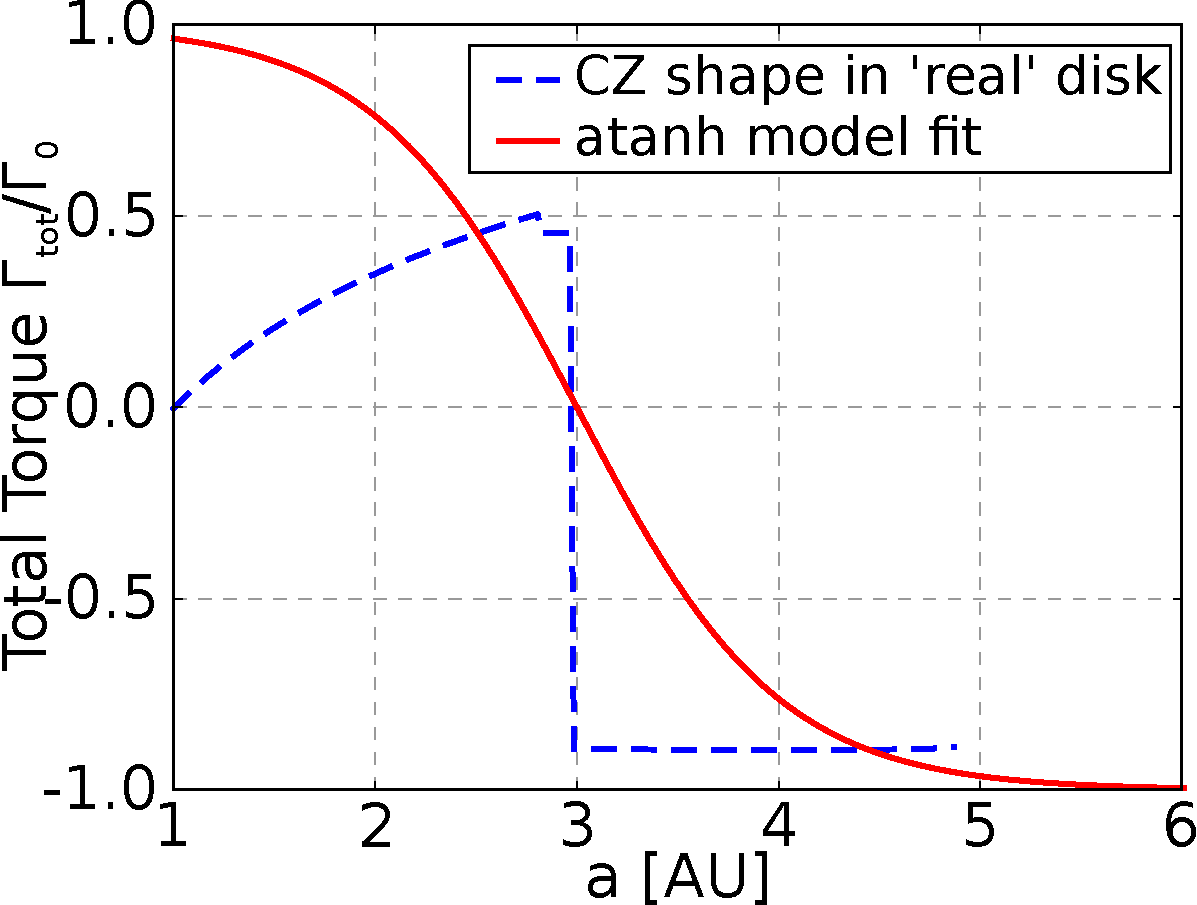
\includegraphics[width=0.49\linewidth]{figure/shifted/torque_zoom_CZ1.pdf}
\caption{Le couple total de notre disque standard est représenté en rouge. La ligne bleue pointillée représente le profil de couple ressenti par une planète de $10\unit{M_\oplus}$ autour d'une transition d'opacité, calculé à partir des équations de \cite{paardekooper2011torque}.}\label{fig:shifted_CZ_torque_prof}
\end{figure}

À noter qu'une fonction de Heavyside n'a pas été utilisée car la marche d'escalier dans le profil \textit{réel} n'est due qu'au fait que la table d'opacité n'a pas été lissée. On s'attend à ce que la transition soit plus douce dans la réalité.
%TODO arnaud veut que je compare une version lissée avec mon tangente hyperbolique.

La position de la zone de convergence était $3\unit{UA}$. À l'intérieur de $3\unit{UA}$, le couple est positif et égal à $\Gamma_0 = \left(\frac{q}{h}\right)^2\Sigma_p {r_p}^4 {\Omega_p}^2$., la migration se fait donc vers l'extérieur. Au delà de $3\unit{UA}$, le couple total est égal à $-\Gamma_0$. Ici $q$ est le rapport entre les masses de la planète et de l'étoile, $h$ est le rapport d'aspect qui dépend du profil de température mais vaut typiquement $0.05$. $\Sigma_p$, $r_p$ et $\Omega_p$ sont respectivement la densité de surface, la distance orbitale et la vitesse angulaire pour la planète. 

Le couple total est la somme du couple différentiel de Lindblad $\Gamma_L$ --- que l'on suppose constant et indépendant de $e$ --- et le couple de corotation $\Gamma_C$. Le principal intérêt de la zone de convergence artificielle est de s'affranchir de la forme très complexe du profil réel et ne garder que la zone de convergence, afin d'en étudier les effets de manière isolée.

\bigskip

\cite{bitsch2010orbital} montrent que la structure de la zone fer-à-cheval est modifiée quand l'excentricité augmente. En conséquence, son couple de corotation $\Gamma_C$, lié à cette région du disque, diminue. 

Nous avons élaboré une formule simple qui reproduit l'effet de l'excentricité sur $\Gamma_C$ par une simple calibration des simulations 3D de \cite{bitsch2010orbital} : 
\begin{align}
D &= \frac{\Gamma_C(e)}{\Gamma_C (e=0)} = 1 + a \cdot \left[\tanh(c) - \tanh\left(\frac{b * e}{x_s}+c\right)\right]\label{eq:shifted-eccentricity-influence}
\end{align}
où $x_s$ représente la demi-largeur de la région fer-à-cheval en unité de distance orbitale de la planète considérée, $e$ est l'excentricité de la planète, et notre ajustement statistique donne les valeurs suivantes pour les paramètres de la fonction :
\begin{align}
a &= 0.45 & b &= 3.46 & c &= -2.34
\end{align}

On défini $x_s$ comme \citep[eq. (44)]{paardekooper2010torque} :
\begin{align}
x_s &= \frac{1.1}{\gamma^{1/4}} \left(\frac{0.4}{b/h}\right)^{1/4} \sqrt{\frac{q}{h}}
\end{align}
où $\gamma$ est l'indice adiabatique, $q$ le rapport entre les masses de la planète et de l'étoile, $h$ le rapport d'aspect et $b/h$ la longueur de lissage du potentiel gravitationnel de la planète (dépendance issue des formules de \cite{paardekooper2011torque}).
%TODO c'est pas uniquement un problème numérique, c'est aussi un problème physique. Voir pour cela paardekooper et papaloizou 2009 ou encore kley & muller 2012
%TODO en gros, de ce que je comprends, il y a le problème de la masse ponctuelle de la planète qui génère une divergence quand on veut calculer la forme des ondes de densité générées par la planète sur le disque. Mais il y a aussi le problème de la longueur de lissage du potentiel du disque quand on veut calculer le couple du disque sur la planète. Il y a donc techniquement deux longueurs de lissages différentes. On doit choisir une seule longueur de lissage pour le potentiel gravitationnel, mais il y a deux longueurs de lissages "optimisées" si on veut faire le calcul d'audrey, JM ou arnaud proprement ; prescription de la longueur de lissage)

\reffig{fig:shifted_CZ_D_profile} montre que notre formule simple \refeq{eq:shifted-eccentricity-influence} correspond bien à la tendance des simulations hydrodynamiques de l'effet de $e$ sur $\Gamma_C$, en particulier pour les excentricités faibles. Il faut tout de même noter qu'il y a peu de points \og expérimentaux\fg et qu'il semble y avoir des fluctuations aléatoires influençant les valeurs mesurées.

\begin{figure}[htb]
\centering
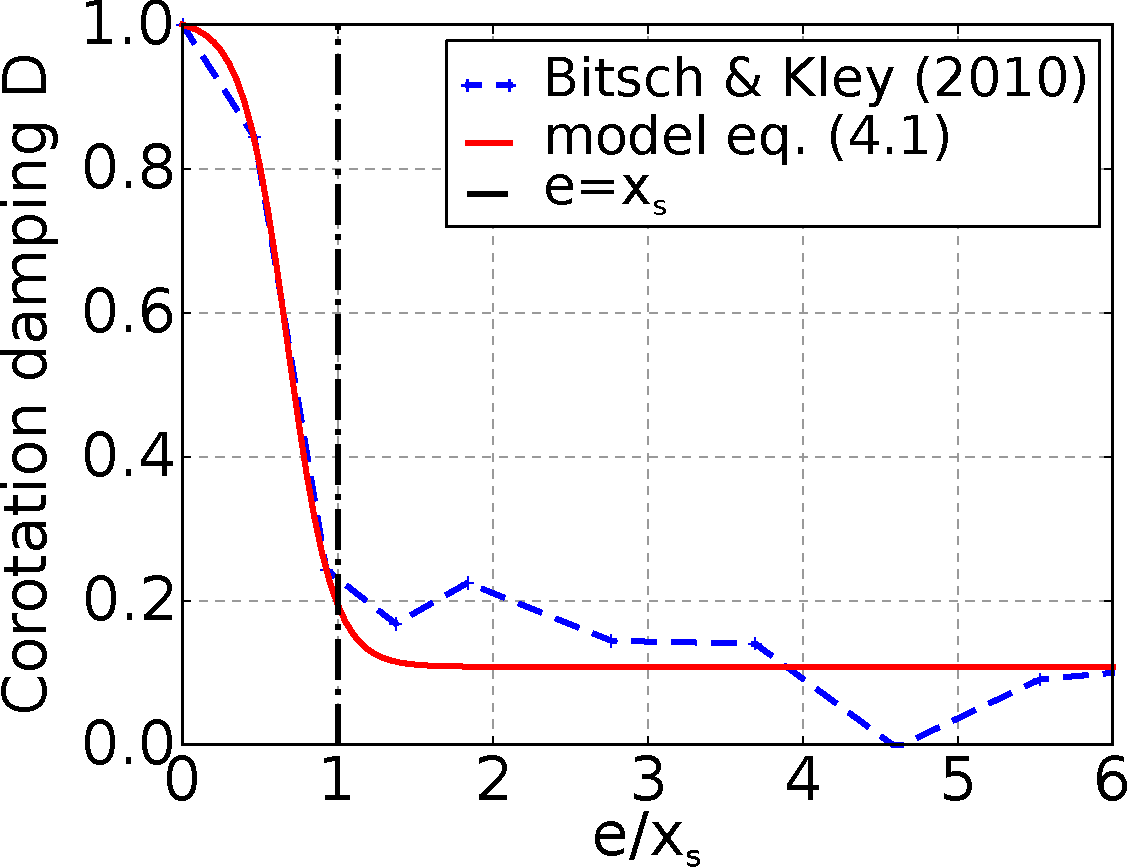
\includegraphics[width=0.49\linewidth]{figure/shifted/corotation_damping_profile.pdf}
\caption{Diminution du couple de corotation $\Gamma_C$ en fonction de l'excentricité $e$. On suppose que l'atténuation ($0<D<1$) du couple de corotation en fonction de l'extencité $e$ est la même dans un disque isotherme ou radiatif. Ainsi, on extrait la valeur de $D$ à partir de la figure 2 de \cite{bitsch2010orbital} en faisant la différence entre la valeur pour le disque radiatif et celle pour le disque isotherme, et normalisant de sorte que $D$ vale $1$ dans le cas $e=0$.}\label{fig:shifted_CZ_D_profile}
\end{figure}

\bigskip

Afin de réaliser nos simulations, nous avons utilisé la version modifiée de l'intégrateur \textbf{Mercury}\citep{chambers1999hybrid} décrite \refsec{sec:code_n-corps}. Nous avons utilisé en particulier la zone de convergence artificielle décrite \reffig{fig:shifted_CZ_torque_prof}. 

Nous supposons que le disque possède le profil de densité de surface suivant :
\begin{align}
\Sigma(R) = 500 \left(R/1\unit{AU}\right)^{-1/2} \unit{g.cm^{-2}}
\end{align}
Ce profil est alors utilisé dans le calcul de $\Gamma_0$ et de l'amortissement induit par le disque sur $e$ et $I$.

Pour implémenter la migration induite par le couple du disque $\Gamma$, on note que $\Gamma=\od{J}{t}$, et on défini une accélération de migration $a_m$ telle que\citep[eq. (14)]{cresswell2008three} :
\begin{align}
a_m &= - \frac{v}{t_m}
\end{align}
où $v$ est la vitesse de la planète et $t_m=J/\od{J}{t}$ le temps de migration ($J$ est le moment cinétique).

\bigskip

Dans toutes les simulations, les planètes était initialement sur des orbites à faible excentricité ($e<0.001$) et faible inclinaison ($I<1^\circ$). Chaque simulation a été intégrée pendant trois millions d'années, avec un pas de temps compris entre $0.4$ et $3$ jours.

\subsection{Le cas de deux planètes}
\reffig{fig:two-planets} montre l'évolution de deux planètes de $1\unit{M_\oplus}$ initialement placées de part et d'autre d'une zone de convergence située à $3\unit{UA}$. Alors qu'elles se rapprochent l'une de l'autre, les deux planètes croisent une série de résonances and finissent piégées dans la résonance \MMR{7}{6}. Les excentricités des deux planètes atteignent alors un équilibre entre excitation résonante et amortissement par le disque. Cette excentricité d'équilibre est environ égale à $0.5$ fois la demi-largeur de la zone fer-à-cheval $x_s$ et amortit le couple de corotation à environ $80\%$ de sa valeur nominale (quand $e=0$). 

\begin{figure}[htb]
\centering
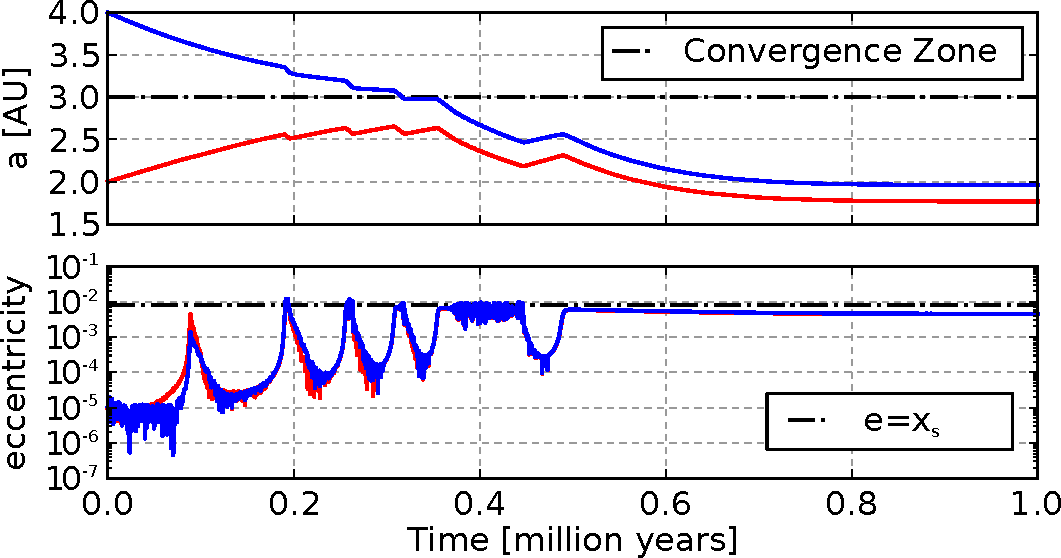
\includegraphics[width=\linewidth]{figure/shifted/corotation_damping_influence.pdf}
\caption{Simulation de la migration convergence de deux planètes de $1\unit{M_\oplus}$ vers la zone de convergence située à $3\unit{UA}$, la rétroactio de l'excentricité $e$ sur le couple de corotation $\Gamma_C$ étant incluse (voir Figure~\ref{fig:shifted_CZ_D_profile}).}
\label{fig:two-planets}
\end{figure}

Les planètes se stabilisent et arrêtent de migrer à $1.77$ et $1.96\unit{UA}$, toutes les deux à l'intérieur de la position nominale de la zone de convergence. Compte tenu de leurs excentricités, la zone de convergence de la planète la plus interne est décalée à $1.95\unit{UA}$ tandis qu'elle est décalée à $1.74\unit{UA}$ pour la planète externe (située à $1.96\unit{UA}$). On constate alors qu'aucune des deux planètes n'est à une position d'équilibre. Chacune d'elle ressent un couple dirigé vers l'autre planète du système, de sorte que la migration tend à rapprocher les planètes tandis que les résonances les maintiennent éloignées.

Le décalage de la zone d'équilibre provient ici de l'équilibre nouveau entre le couple de Lindblad resté inchangé et le couple de corotation atténué par l'excentricité. \emph{Les deux planètes se stabilisent autour d'une zone où le couple total exercé sur le système dans sa globalité est nul, même si chaque planète prise séparément ressent un couple de migration non nul}. Aucune des deux planètes n'est ici à une zone de convergence (même celle calculée en tenant compte de l'atténuation du couple de corotation). 

Il est clair que les excentricités des planètes --- excitées par les interactions entre planètes --- sont le facteur clé pour déterminer la force du couple de corotation et la position effective de la zone de stabilisation du système. Pour deux planètes de même masse, le même comportement qualitatif est observé, quelle que soit la masse ou la résonance considérée : Une plus grande excentricité implique un amortissement plus fort du couple de corotation $\Gamma_C$ et une stabilisation du système de plus en plus proche de leur étoile. 

\subsection{Effet du rapport de masse}\label{sec:mass-ratio-effect}
Nous étudions maintenant le cas de deux planètes de masses différentes. \reffig{fig:mass_ratio_final_pos} représente les positions finales d'une série de simulations simples dans lesquelles une planète de $10\unit{M_\oplus}$ est placée systématiquement à $3\unit{UA}$ en compagnie d'une autre planète, placée à $4\unit{UA}$ et dont la masse varie successivement entre $0.1$ et $3\unit{M_\oplus}$. 

\begin{figure}[htb]
\centering
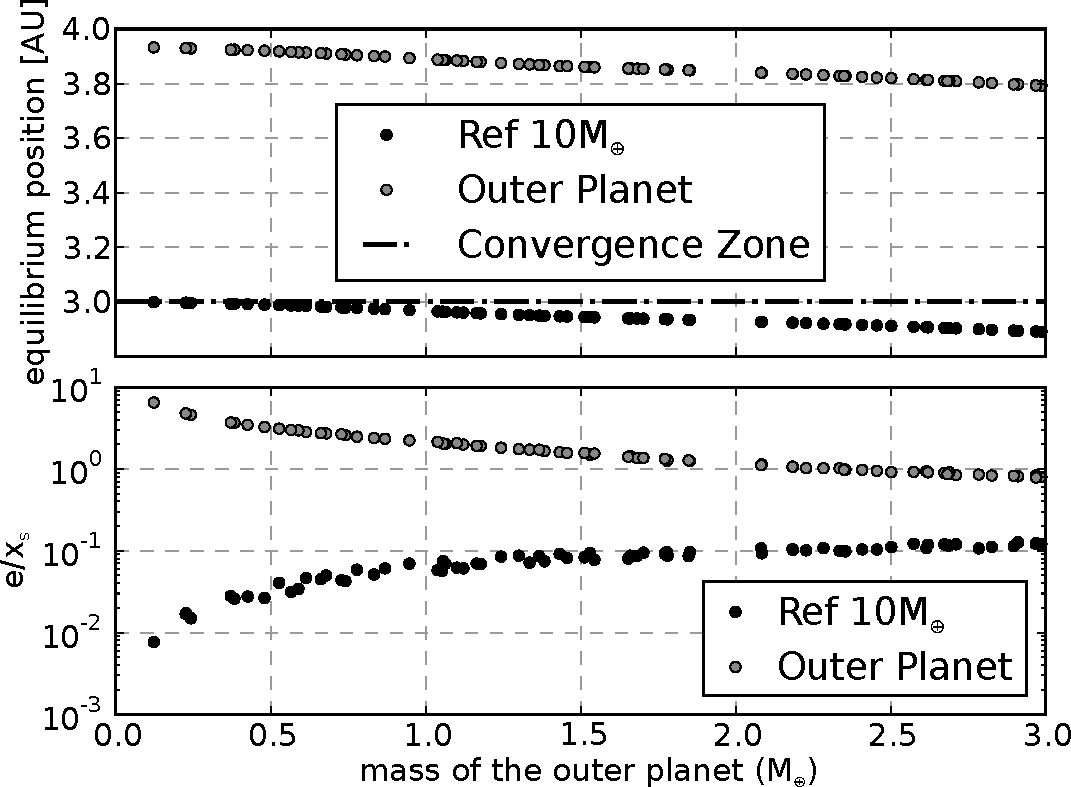
\includegraphics[width=0.95\linewidth]{figure/shifted/mass_ratio_influence.pdf}
\caption{Système final d'une série de simulations avec initialement une première planète à $3\unit{UA}$ de $10\unit{M_\oplus}$ et une deuxième planète à $4\unit{UA}$ dont la masse varie de $0.1$ à $3\unit{M_\oplus}$. Les graphiques montrent la position d'équilibre des planètes (en haut) et les excentricités normalisées par rapport à la demi-largeur de la zone fer-à-cheval $e/x_s$ (en bas) en fonction de la masse de la deuxième planète.}\label{fig:mass_ratio_final_pos}
\end{figure}

\bigskip

Dans \reffig{fig:mass_ratio_final_pos}, la planète externe est systématiquement en résonance \MMR{3}{2} avec la planète interne. Ainsi, la position finale des planètes est déterminée par leur masse respective ou, pour cette expérience, par la masse de la planète externe vu que la masse de la planète interne est fixe. 

Plus la deuxième planète est massive, et plus le décalage du système planétaire par rapport à la zone de convergence est important. En effet, une planète externe plus massive induit une excentricité plus importante pour la planète interne, ce qui correspond à un amortissement plus important de son couple de corotation $\Gamma_C$ et un décalage plus important de la zone d'équilibre du système. Compte tenu du fait que chaque planète possède une masse et une excentricité différentes, elles ressentent une zone de convergence différente (une pour chaque valeur de $e/x_s$). Pour autant, l'importance du décalage vers l'étoile centrale de la position d'équilibre est principalement déterminée par la dynamique de la planète la plus massive et de sa nouvelle zone de convergence.

\bigskip

\reffig{fig:mass_ratio_final_pos} représente uniquement un sous-ensemble de toutes les simulations de cette expérience. Pour des masses plus importantes, les deux planètes étaient dans des résonances différentes, ce qui causait des discontinuités dans le diagramme, rendant difficile sa lecture. Malgré tout, le comportement du système de deux planètes est qualitativement le même.

\subsection{Effet des résonances}
Dans la position d'équilibre d'un système de deux planètes, l'ordre de la résonance entre les deux corps est aussi important (pour une résonance de moyen mouvement \MMR{(p+q)}{p}, $p$ est l'ordre de la résonance). 
%TODO demander à Sean pour ça. Arnaud me dit que l'ordre, c'est q, et que p est le degré de la résonance.

Deux planètes en résonance \MMR{3}{2} auront des excentricités plus importantes que si elles étaient en résonance \MMR{11}{10}. L'explication simple est qu'une résonance d'ordre moins élevé implique des conjonctions plus fréquentes, et ainsi des perturbations plus importantes (voir \cite{murray2000solar} pour plus de détails). La résonance dans laquelle un système de deux planètes se place dépend de la vitesse de migration relative et du taux d'amortissement de l'excentricité par le disque (voir par exemple \cite{mustill2011general}). Ces deux derniers paramètres sont déterminés à la fois par le disque, le profil de couple et les positions initiales des planètes. 

\begin{figure}[htb]
\centering
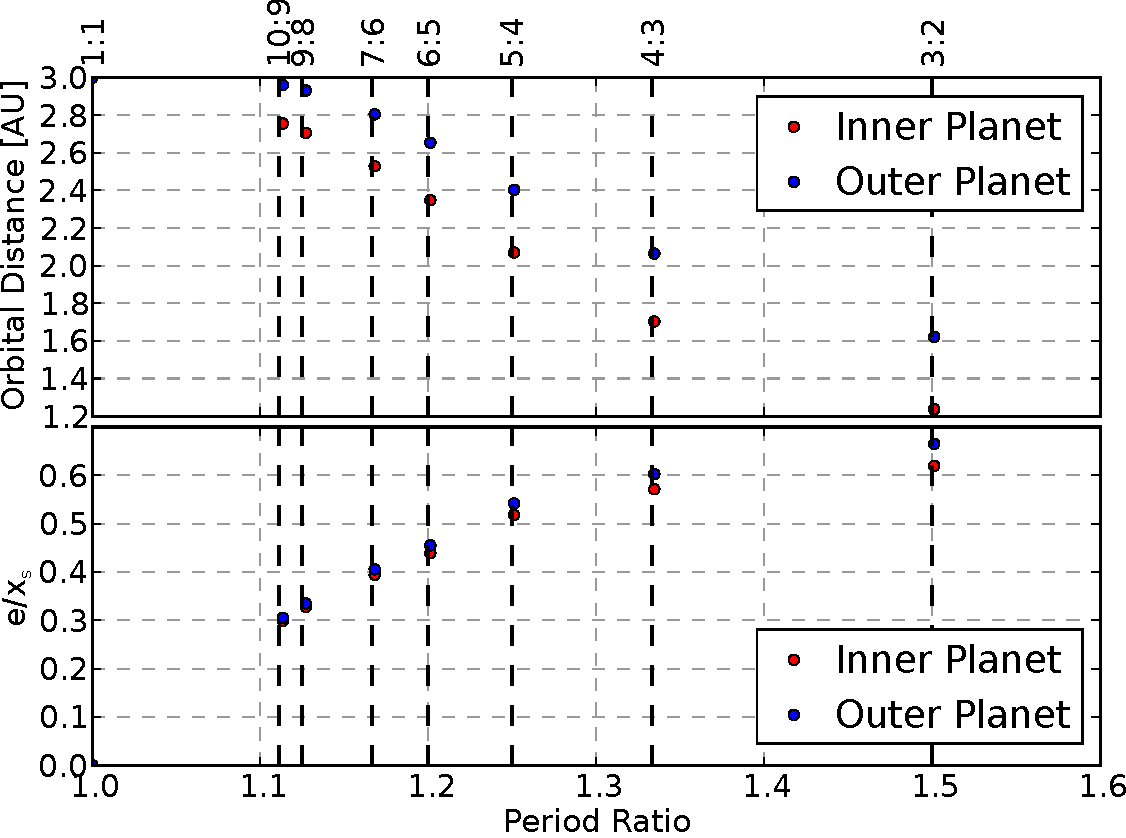
\includegraphics[width=0.95\linewidth]{figure/shifted/influence_of_MMR.pdf}
\caption{demi-grand axe final (en haut) et excentricité (en bas) de deux planètes de $3\unit{M_\oplus}$ piégées dans différentes résonances de moyen mouvement. Pour une planète de $3\unit{M_\oplus}$, la demi-largeur de la zone fer-à-cheval vaut environ $0.014$.}\label{fig:influence_of_MMR}
\end{figure}

Afin de tester l'effet des résonances, nous avons fait une série de 100 simulations (chacune intégrée pour un million d'années), avec deux planètes de $3\unit{M_\oplus}$ placés aléatoirement entre 1 et 10 UA, avec la même zone de convergence artificielle placée à 3 UA que précédemment. 

\reffig{fig:influence_of_MMR} montre que dans tous les cas, les planètes sont bloquées dans des résonances allant de \MMR{11}{10} à \MMR{3}{2} (ordre de la résonance de 10 à 2). Conformément à ce qui était attendu, les excentricités maintenues grâce aux résonances diminuent à mesure que l'ordre des résonance augmente, et ceci induit un décalage moins important du système planétaire par rapport à la zone de convergence à 3 UA. L'amplitude du décalage vers l'intérieur de la position d'équilibre varie de 0.2 à 1.5 UA. 

Dans deux simulations, les planètes ont commencé si proches l'une de l'autre qu'elles se sont retrouvé en résonance co-orbitale (résonance \MMR{1}{1}). Dans ces cas là, leurs excentricités sont restées très faibles, et les deux planètes ont migré en co-orbite jusqu'à la zone de convergence nominale à 3 UA. 

\subsection{Évolution avec plus de deux planètes}
On se concentre maintenant sur le cas multi-planètes. Nous avons lancé 10 simulations pour des cas avec deux, trois, cinq ou dix planètes, initialement toutes de $3\unit{M_\oplus}$. Les planètes étaient placées aléatoirement entre 1 et 10 UA, et étaient sur des orbites de faible inclinaison et excentricité. Comme précédemment, chaque simulation a été intégrée pendant trois millions d'années dans un disque statique (sans dissipation). 

\bigskip

Dans les cas avec 3 planètes, on trouve 3 scénarii différents. Dans un premier cas, les 3 planètes sont prises dans une chaine de résonance et migrent vers l'intérieur toutes ensemble jusqu'à une zone d'équilibre où le couple total exercé sur le système est nul. Cette zone est typiquement entre 2 et 2.5 UA. Les excentricités des trois planètes ne sont pas identiques, la planète au centre de la chaîne de résonance est généralement la plus excitée. 

Dans le deuxième scénario le plus probable, deux planètes entrent en résonance et migrent vers l'intérieur tandis que la troisième et dernière planète est trop loin dans le disque pour être elle aussi prise en résonance avec les deux autres. Cette dernière planète migre alors à la zone de convergence à 3 UA, tandis que les deux planètes internes stoppent leur migration autour d'une zone d'équilibre où le couple total exercé sur le système est nul. 

Enfin, dans un troisième scénario, une collision a lieu et le système revient à un cas à deux planètes de masse différente comme vu précédemment \reffig{fig:mass_ratio_final_pos}. 

\bigskip

Pour les cas à 5 et 10 planètes, la situation est plus complexe. Les systèmes de 5 planètes forment des chaines de résonances et migrent vers l'intérieur, en direction d'une position d'équilibre où le couple total est nul. Cependant, les perturbations entre planètes ajoutent un aspect erratique à la migration des planètes. Même les systèmes les plus stables subissent des périodes d'instabilités durant lesquelles les planètes dérivent radialement dans la même direction. Ces périodes sont déclenchées par la sortie d'une résonance d'un couple de planètes à l'intérieur du système. Cette sortie de résonance se propage alors comme une perturbation à travers tout le système. L'amplitude et la fréquence de ces périodes chaotiques varient d'une simulation à l'autre. 

%\begin{figure}[htb]
%\centering
%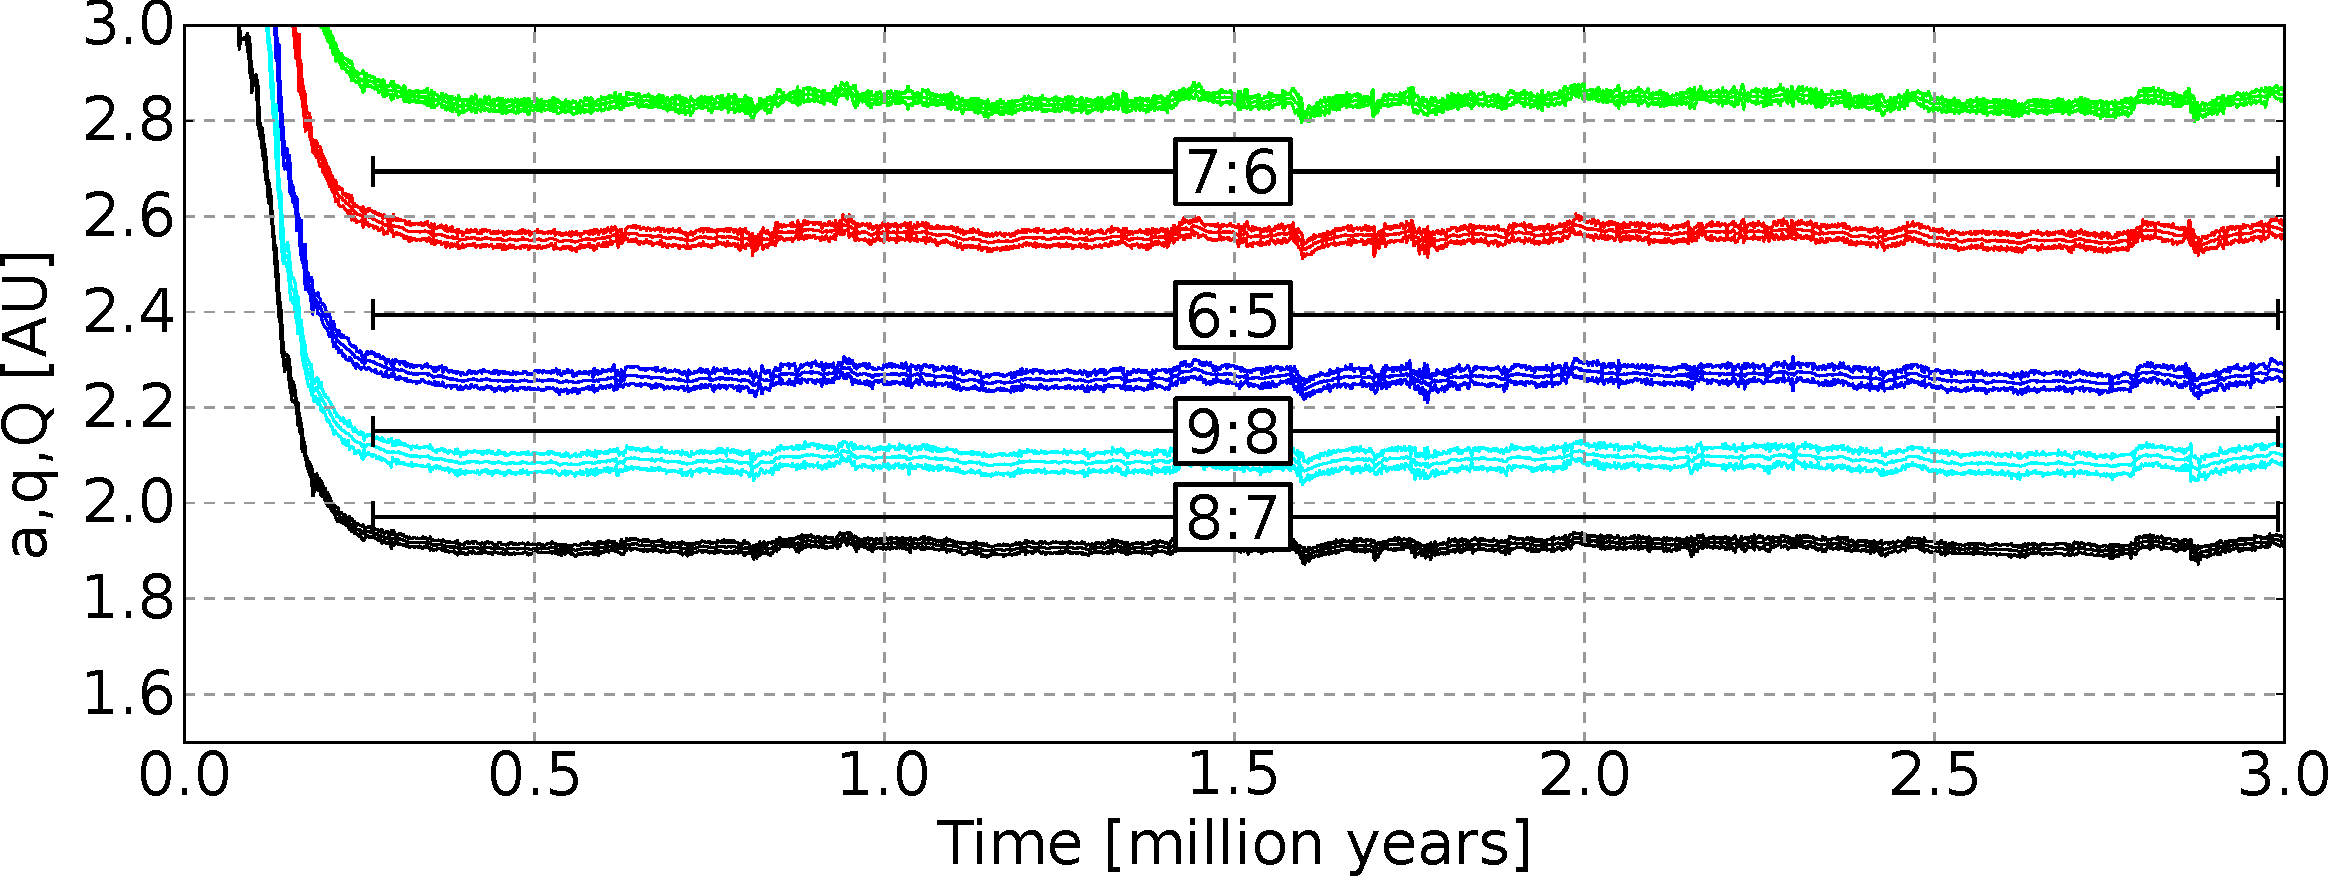
\includegraphics[width=\linewidth]{figure/shifted/5_simu00009_stable.pdf}\\
%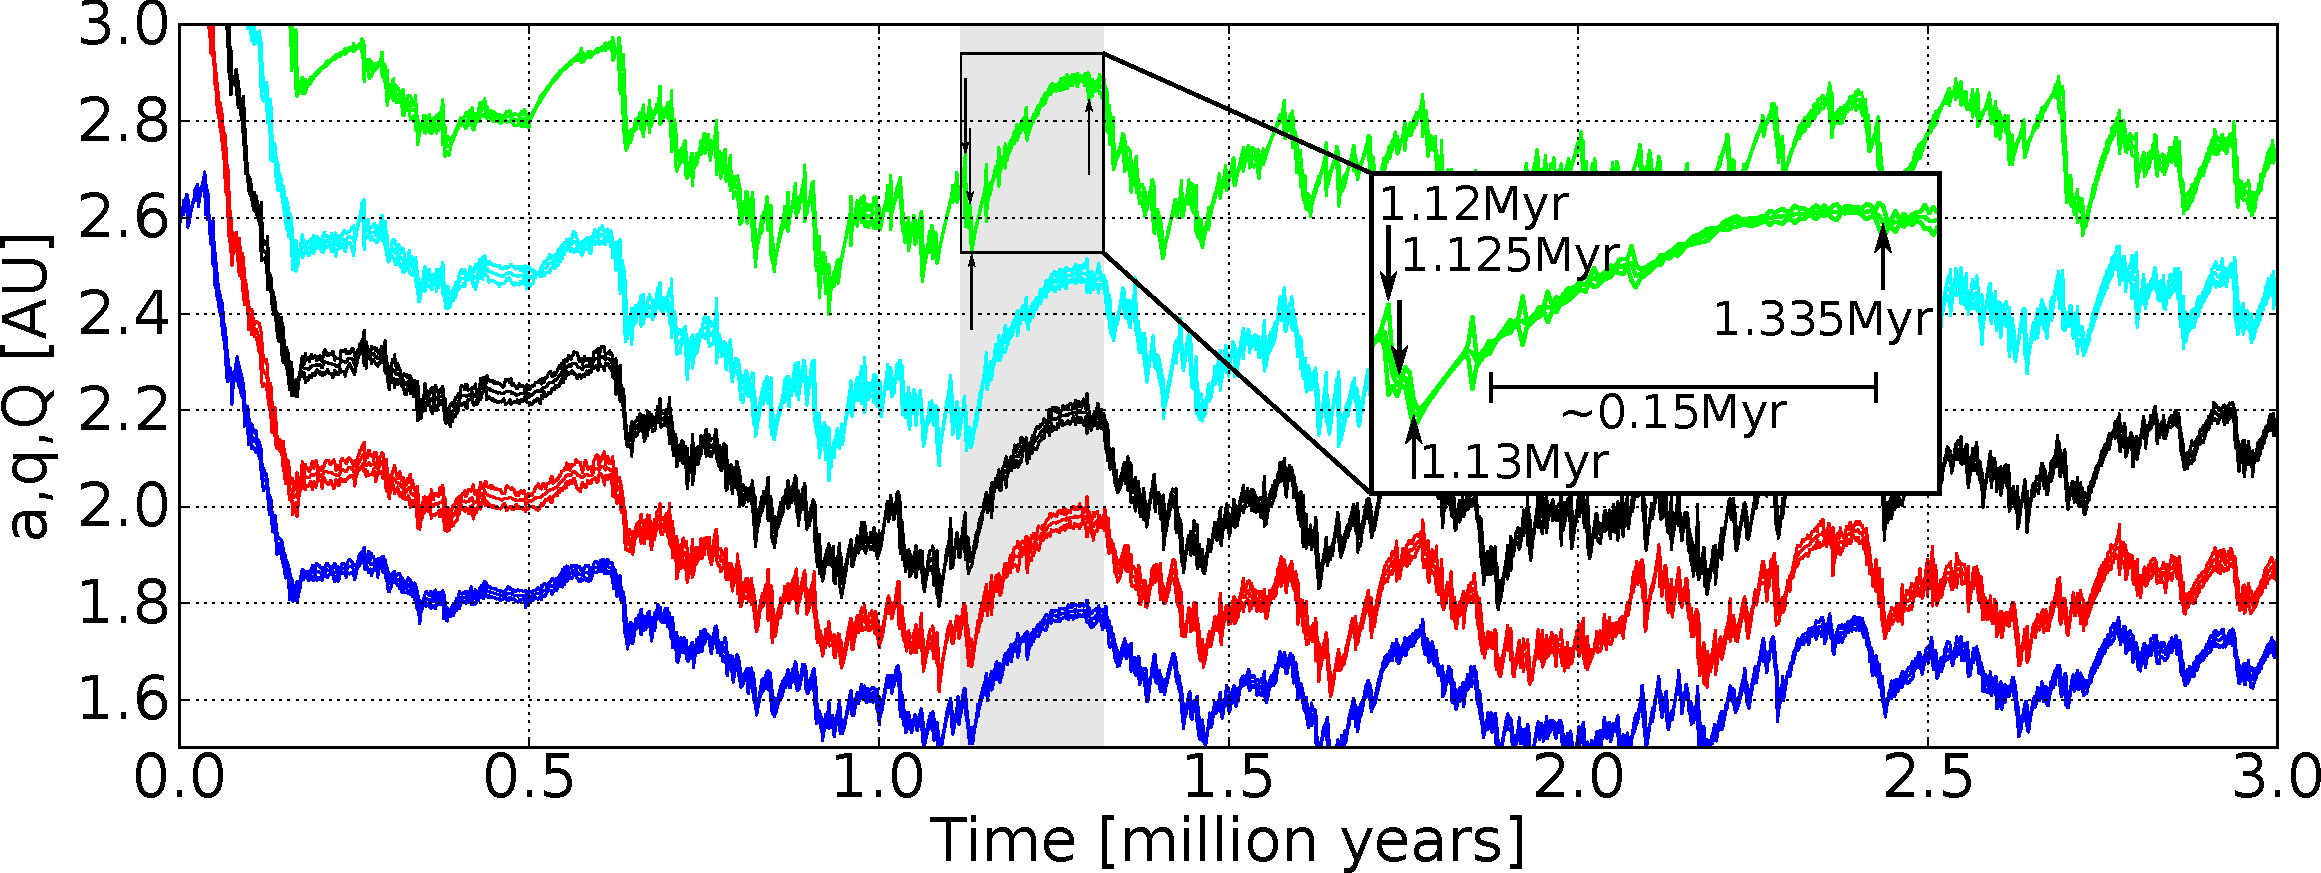
\includegraphics[width=\linewidth]{figure/shifted/5_simu00010_unstable.pdf}
%\caption{Deux exemples de simulations avec 5 planètes, une qui est relativement stable, même si de courts épisodes de pertubations des résonances ont lieu (en haut) et une qui possède un comportement chaotique soutenu (en bas).}
%\label{fig:timed-resonance-unstable}
%\end{figure}

\begin{figure}[htb]
\centering
\subfloat[Simulation relativement stable, même si de courts épisodes de pertubations des résonances ont lieu]{\label{fig:timed-resonance-stable}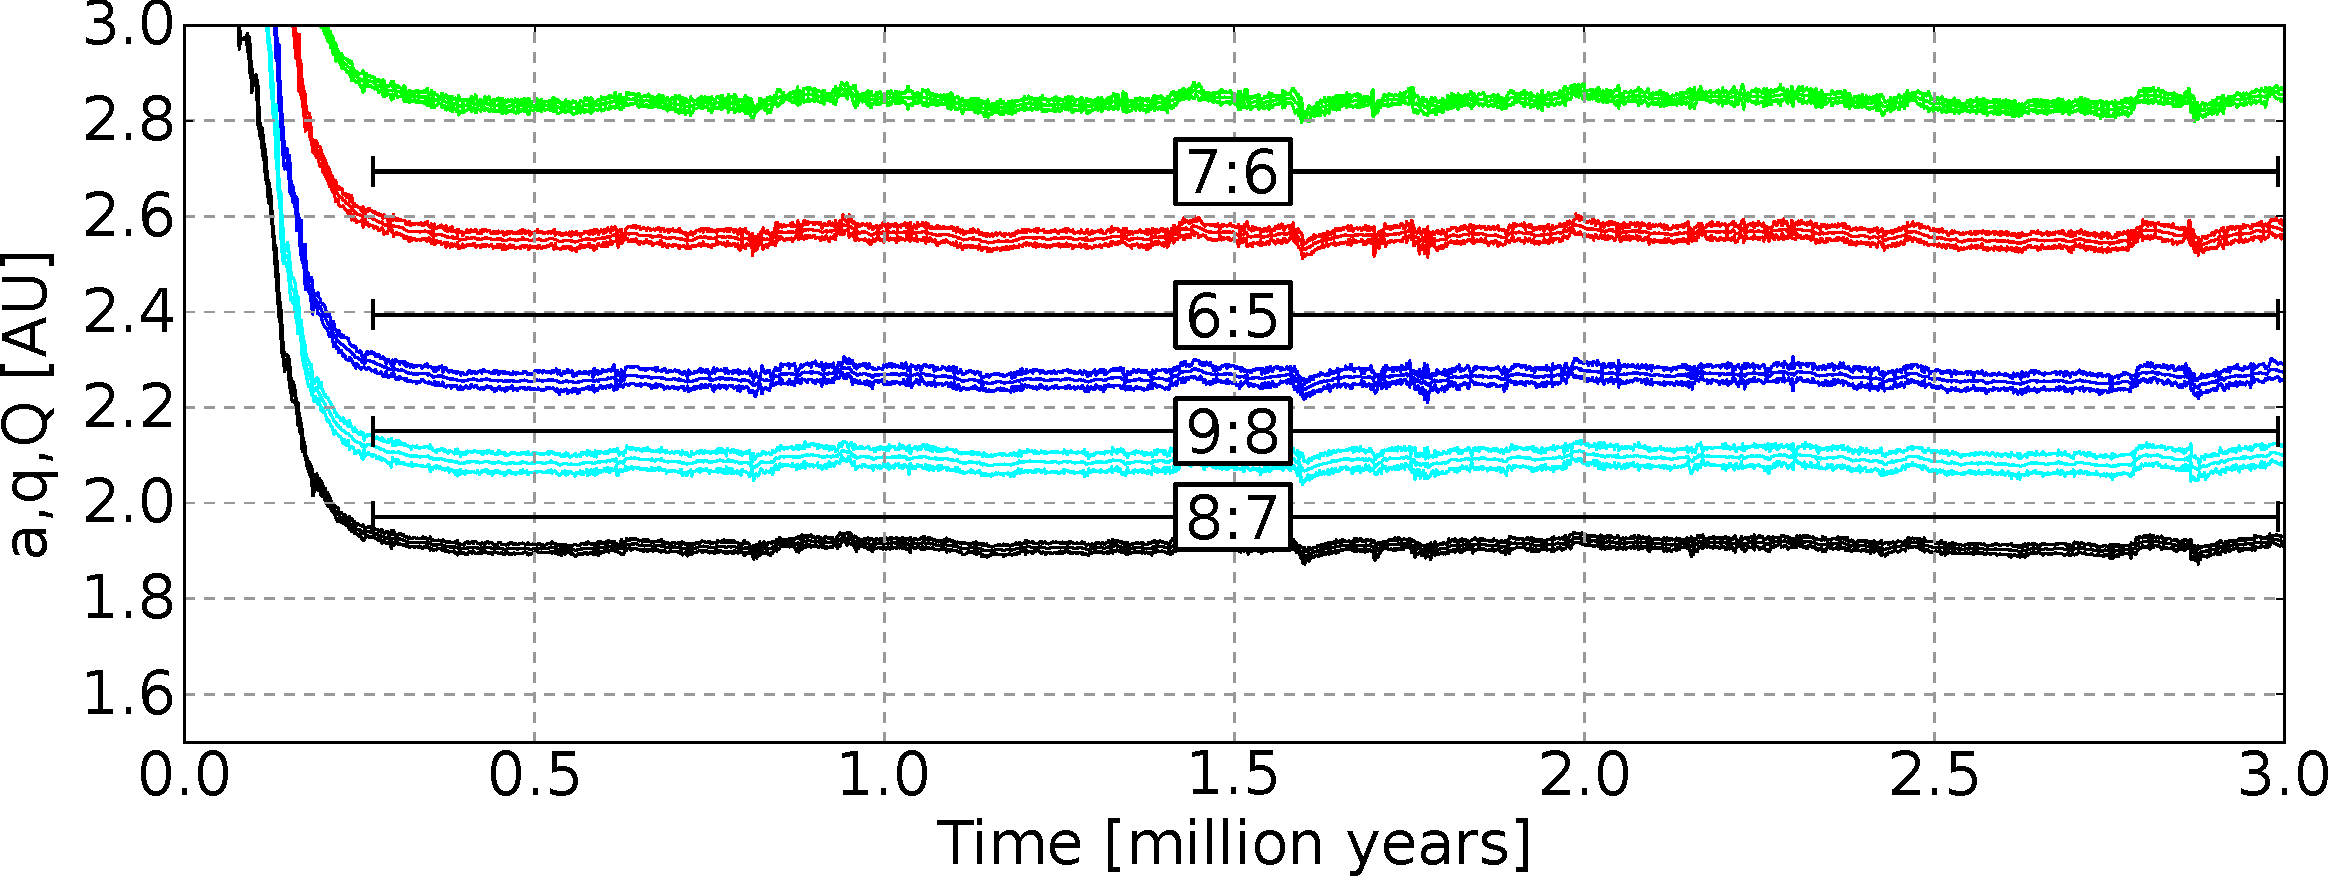
\includegraphics[width=\linewidth]{figure/shifted/5_simu00009_stable.pdf}}\\
\subfloat[Simulation qui possède un comportement chaotique soutenu]{\label{fig:timed-resonance-unstable}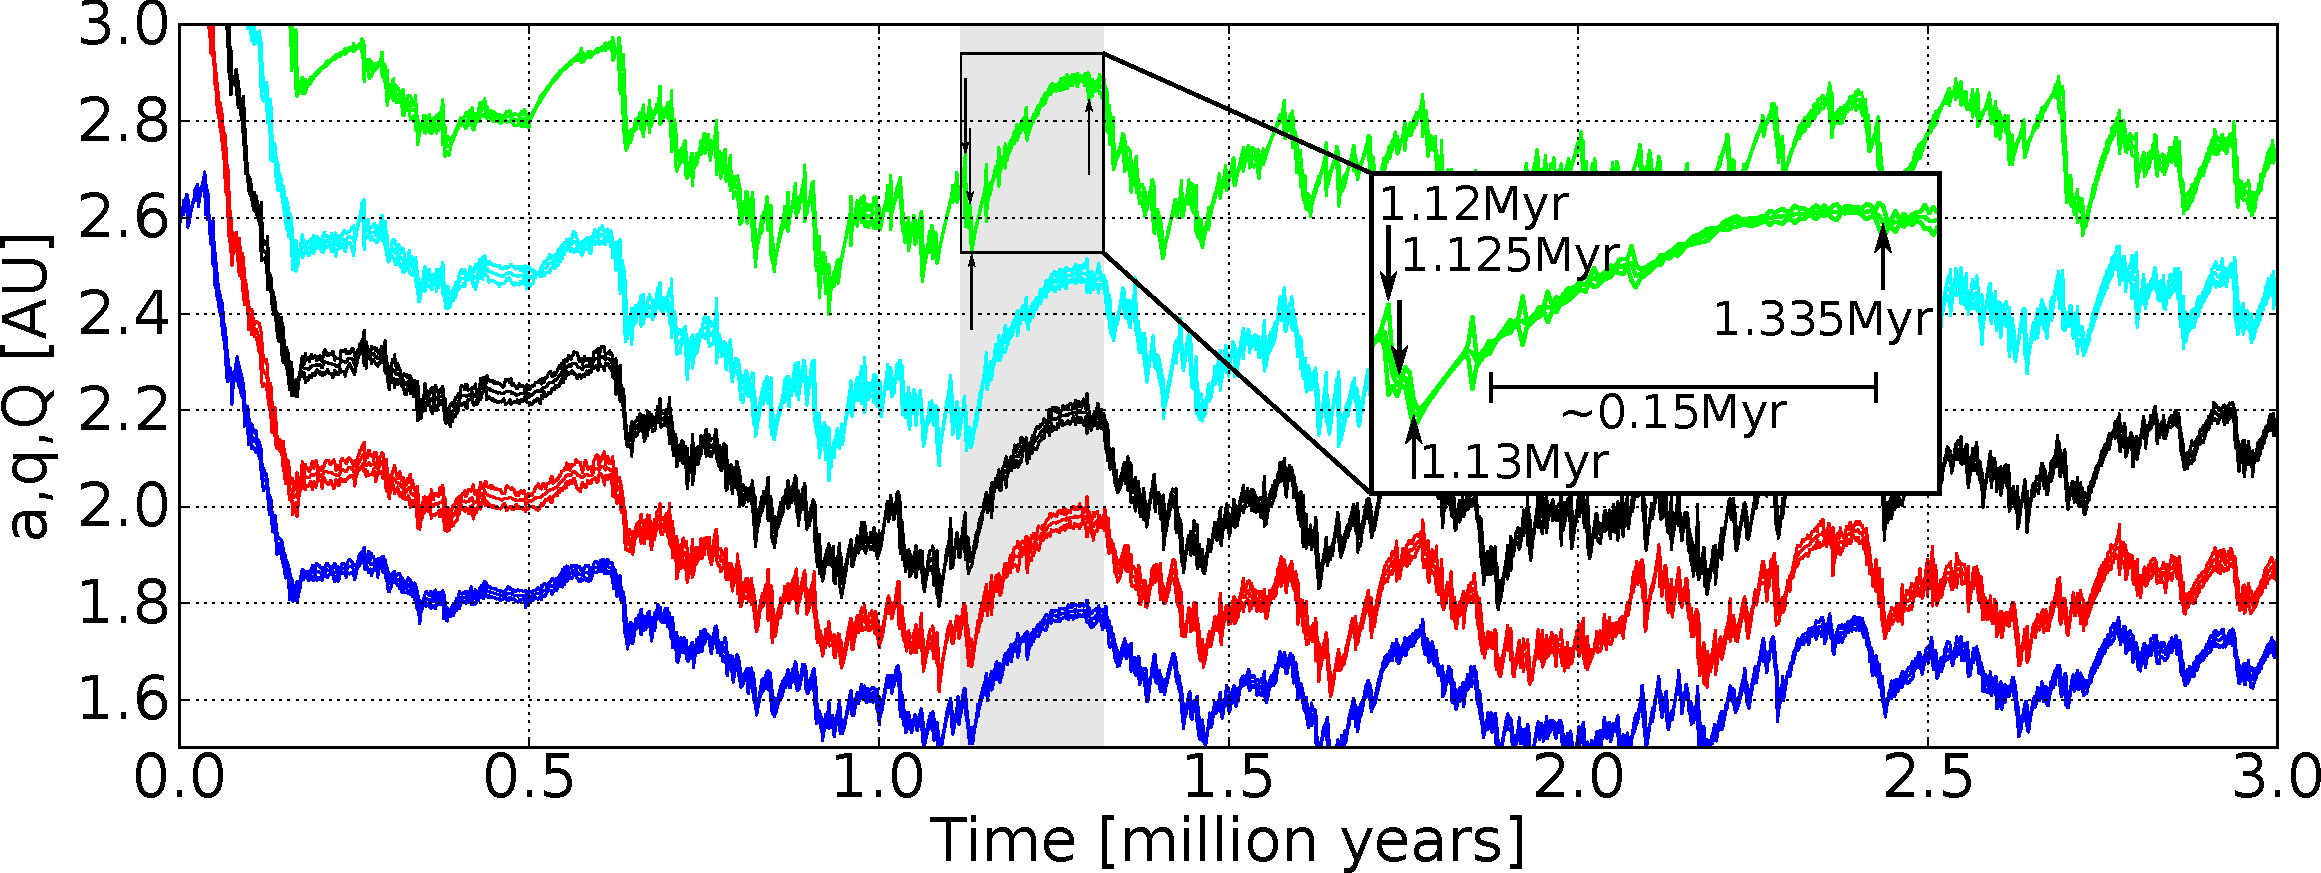
\includegraphics[width=\linewidth]{figure/shifted/5_simu00010_unstable.pdf}}
\caption{Deux exemples de simulations avec 5 planètes}\label{fig:timed-resonance-stability}
\end{figure}

Par exemple, dans la simulation \reffig{fig:timed-resonance-stable}, la chaine de  résonance subit plusieurs petites perturbations sans grandes conséquences car leur amplitude est faible devant la distance entre les planètes. Par opposition, les perturbations de la simulation  \reffig{fig:timed-resonance-unstable} sont bien plus importantes.

Considérons en particulier l'épisode chaotique entre 1.1 et 1.3 million d'années dans le cas décrit \reffig{fig:timed-resonance-unstable}. À 1.12 million d'années, les deux planètes externes sont piégées dans une résonance orbitale \MMR{4}{3}. Elles migrent alors vers l'intérieur, à cause de la soudaine excitation de leurs excentricités via la résonance. Cette perturbation se propage alors vers le système interne, et les excentricités de toutes les planètes augmentant soudainement, le système total se met peu à peu à migrer entièrement vers l'intérieur. 5000 ans plus tard, les deux planètes externes, encore les mêmes, sortent puis entrent de nouveau en résonance \MMR{4}{3}, perturbant de nouveau le système. Finalement, à 1.13 million d'années, les deux planètes externes sortent définitivement de la résonance \MMR{4}{3}. Retrouvant leur liberté de corps isolé, les deux planètes migrent vers la zone de convergence avec leurs excentricités de nouveau quasi nulle, la résonance n'étant plus là pour maintenir les 
excentricités face à l'amortissement du disque.

Sans le couple négatif des deux planètes externes, l'équilibre des couples du système global est modifié. En réaction, le système interne de trois planètes migre vers l'extérieur vers une nouvelle zone d'équilibre où le couple total exercé sur le système de trois planètes est nul. Ceci explique alors pourquoi les 5 planètes migrent brutalement vers l'extérieur. 

Cependant, les deux planètes externes entrent rapidement en résonance \MMR{5}{4}. Pendant les quelques 0.15 million d'années suivants, elles entrent périodiquement en résonance \MMR{5}{4} mais la migration vers l'extérieur continue car la plupart du temps elles ne sont pas en résonance et leur excentricité reste relativement faible. La migration globale vers l'extérieur du système s'arrête à 1.335 million d'années quand les deux planètes externes traversent la résonance \MMR{5}{4} et sont piégées dans la résonance orbitale \MMR{6}{5}. Cette configuration stabilise le système, excite les excentricités des planètes externes et entraine la migration globale du système tout entier vers l'intérieur, marquant la fin de cet épisode chaotique. 

\bigskip

Le reste de l'évolution est composé du même type de perturbations. Les perturbations proviennent des planètes qui entrent ou sortent des résonances, et qui se propagent alors au reste du système. 

Quand les planètes sortent de résonance, leur excentricité décroit rapidement, entrainant une migration vers l'extérieur. Par opposition, les planètes entrant en résonance voient leur excentricité croitre et être maintenue à un niveau constant non nul qui entraine une migration vers l'intérieur. 

Au travers de ces perturbations, des systèmes entiers subissent des migrations chaotiques relativement modestes qui illustrent la difficulté pour le système de maintenir une chaine de résonance pendant de longues périodes. 

La totalité des systèmes de 5 planètes que nous avons modélisés est restée stable, dans le sens où aucune collision n'a eu lieu. Mais l'amplitude de la migration chaotique subie par le système varie d'un système à l'autre. Les deux exemples de \reffig{fig:timed-resonance-stability} montrent les deux cas les plus extrêmes. Les simulations avec 10 planètes étaient encore plus chaotiques et des collisions ont eu lieu. 

\bigskip

Le point le plus important pour déterminer l'amplitude des oscillations chaotiques d'un système est l'ordre des résonances. Des résonances d'ordre $p$ faible (par exemple \MMR{3}{2}) maintiennent des excentricités élevés et sont moins stables car elles sont sensibles aux variations d'excentricité. Dans le même temps, les résonances d'ordre $p$ élevé (par exemple \MMR{11}{10}) maintiennent des excentricités plus faibles et sont moins sensibles aux perturbations d'excentricité.

Par exemple \reffig{fig:timed-resonance-stable}, les perturbations sont rapidement amorties tandis que dans le panneau du bas, la fréquence des perturbations est suffisamment importante pour que le système n'ait pas le temps de les amortir et ne tendent donc pas vers une configuration stable. \emph{Dans ce contexte, un système compact est donc plus stable qu'un système plus étendu, ce qui est exactement l'opposé d'une situation purement gravitationnelle} \citep{marchal1982hill}.

\subsection{Discussion}
Au travers de cette partie, nous avons montré que les planètes ne sont pas forcément piégées à la zone de convergence. Au lieu de cela, les embryons migrent rapidement vers la zone de convergence et sont piégés dans des chaînes de résonance. Ceci entraine l'augmentation brutale de leur excentricité qui reste suffisamment importante pour atténuer le couple de corotation. La zone d'équilibre de la chaîne de résonance dans le disque est déterminée par la somme des couples ressentis individuellement par les planètes (chaque terme étant la somme d'un couple de corotation atténué et d'un couple différentiel de Lindblad non atténué). Dans la pratique, cette zone de couple nul effective est déterminée principalement par la zone de convergence décalée de la planète la plus massive de la chaîne de résonance. Ce n'est pas une vraie zone de convergence car chaque planète voit une zone de convergence différente en fonction de son excentricité.

\bigskip

Le décalage vers l'intérieur existe parce que les excentricités des planètes sont maintenues par les perturbations résonantes. L'amplitude de l'excentricité d'une planète est le résultat de la compétition entre l'excitation résonante et l'amortissement de l'excentricité par le disque. Pour des excentricités suffisamment importantes, un système entier de planètes en résonance peut migrer jusqu'au bord interne.

Changer les propriétés du disque pourrait ainsi changer les valeurs typiques des excentricités en modifiant le temps caractéristique d'amortissement des excentricités. Cependant, changer les propriétés du disque a aussi des conséquences sur d'autres grandeurs influençant le système, tel que le profil de couple exercé par le disque sur les planètes. En changeant les propriétés du disque, il n'est pas évident de dire quelles seront les conséquences sur l'évolution des planètes, compte tenu du fait que les planètes pourront être dans des résonances différentes, avec des excentricités et des critères de stabilité différents. 

La zone de convergence dépend des paramètres du disque tels que la viscosité, les profils de température et de densité de surface \citep[voir par exemple][]{paardekooper2011torque}.Ici, nous avons utilisé un profil de disque issu de modèles complexes, mais qui reste malgré tout artificiel. Même si les résultats dépendent d'un modèle particulier, ils sont robustes aux variation du profil de couple en fonction de la distance orbitale, tant qu'une zone de convergence existe pour rassembler les embryons au cours de l'évolution. 

\bigskip

Dans un disque plus réaliste, on s'attend à quelques différences. En premier lieu, il pourrait exister plusieurs zones de convergence dans un même disque ayant pour origine des processus physiques différents \citep{lyra2010orbital, hasegawa2011origin}. 

Ensuite, des zones de convergences dépendantes de la masse des planètes peuvent exister dans les parties externes du disque, où ce mécanisme devrait être moins efficace compte tenu du fait que dans de telles zones de convergence, les embryons de masse différentes ne migrent pas à la même position dans le disque. Dans de telles zones, il pourrait être beaucoup plus difficile de former les chaînes de résonances essentielles pour notre mécanisme.

Troisièmement, alors que le disque se dissipe, le profil de couple et la position des zones de convergences sont aussi altérées \citep{lyra2010orbital, horn2012orbital}. 

Enfin, la turbulence est censée être commune dans les disques protoplanétaires \citep{armitage2011dynamics}. Même si la turbulence n'affecte pas l'évolution à long terme d'une planète isolée dans un disque radiatif \citep{pierens2012protoplanetary}, on s'attend à ce qu'elle modifie la capture en résonance et l'évolution des excentricités \citep[voir][]{pierens2011dynamics}.

\section{Formation des super-Terres chaudes}\label{sec:4.2}
Les détections d'exoplanètes par vitesse radiale et transit montrent que $30$ à $50\%$ des étoiles de la séquence principale possèdent au moins une planète de moins de $10\mearth$ sur des orbites comprises entre $85$ et $100$ jours \citep{mayor2011road, howard2010occurrence, howard2012occurrence, fressin2013false}. De plus, les super-Terres ($1-10\mearth$) chaudes sont préférentiellement détectées dans des systèmes multiples \citep{udry2007statistical, lissauer2011architecture}. Pourtant, même si ces systèmes peuvent nous sembler bien plus compacts que le système solaire au premier abord, d'un point de vue gravitationnel, ils possèdent à peu près le même espacement en terme de rapport de période et de rayon de Hill mutuel \citep{fang2013planetary}.


\reffig{fig:multiplanet_stats} montre les propriétés statistiques des planètes détectées dans des systèmes multiples, incluant les candidats Kepler.%TODO raconter plus de choses sur les stats?

\begin{figure}[htb]
\centering
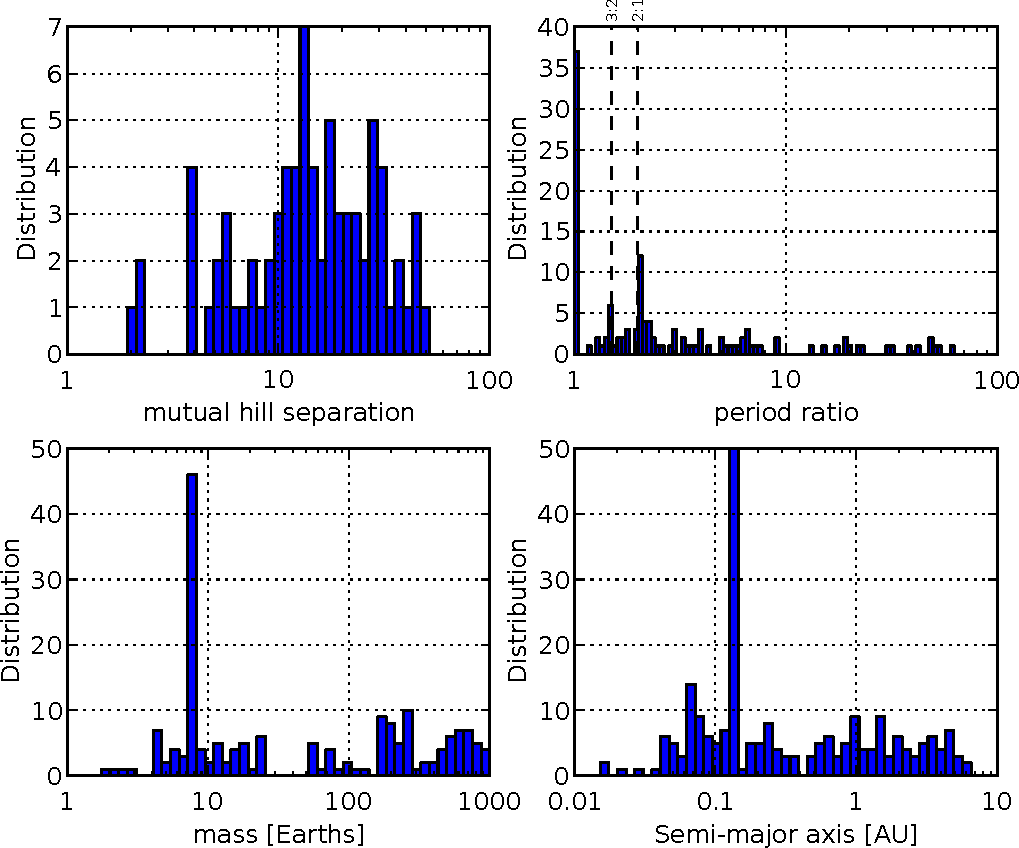
\includegraphics[width=0.8\linewidth]{figure/multiplanet_systems_stats.pdf}
\caption{Propriétés des exoplanètes détectées dans des systèmes multiples ($N\geqslant 2$). Données (01/01/2013) : \url{http://exoplanets.org/}}\label{fig:multiplanet_stats}
\end{figure}

\bigskip

Plusieurs mécanismes de formations tentent d'expliquer la présence de super Terres, ces planètes ayant une masse de $1$ à $10\mearth$, tout en étant compatible avec les contraintes observationnelles. Deux modèles principaux peuvent à ce jour expliquer la formation de ces planètes. 

Le premier modèle, la \og formation \textit{in-situ}\fg \citep{chiang2013minimum} n'est possible que si le disque est suffisamment massif localement pour permettre la formation de planète de plusieurs masses terrestres. La formation est alors semblable à celle des planètes telluriques dans le système solaire \citep{wetherill1990formation, kenyon2006terrestrial}.

Le deuxième modèle implique la migration de type 1 \citep{terquem2007migration}. Dans ce cas là, il n'est pas nécessaire de supposer un disque extrêmement massif afin de former plusieurs super terres. 

Les deux modèles permettent d'expliquer l'espacement observé. Le modèle impliquant la migration de type 1 prédit aussi que les systèmes multiples vont être proches de résonances de moyen mouvement. On peut en effet observer des pics sur \reffig{fig:multiplanet_stats} autour des résonances \MMR{3}{2} et \MMR{2}{1}. Dans le cas de la formation \textit{in-situ}, on s'attend à des planètes assez pauvres en eau, alors qu'en impliquant la migration, la variété de composition des planètes ainsi formées est beaucoup plus grande \citep{raymond2008observable}.

Il existe de plus d'autres modèles, impliquant des résonances séculaires avec des planètes géantes plus loin dans le système, la photo-évaporation de super Neptunes, circularisation des planètes excentriques. Ces modèles sont présentés et comparés dans \cite{raymond2008observable} et ne sont pas discutés ici. 

%TODO 
%Observations : contraintes en fonction de la masse des planètes, séparation (en delta, et en p2/p1)
%
%autres modèles : 
%-in-situ (murray & hansens, ou chiang & laughlin, raymond 2008) il y a un résumé de tous les modèles dans raymond 2008
%-type I migraiton (terquem & papaloizou)
%
%_______
%environ une ou deux page pour cette intro

%TODO parler des raisons de la migration vers l'intérieur (intérieur car faible masse, ou intérieur car corotation damping). 
%TODO Parler aussi de ce qui arrête les planètes au bord interne. Faire des tests pour ça.

\subsection{Modèle}
Nous utilisons les formules de \cite{paardekooper2011torque} afin de modéliser la migration de type I. Cette migration est implémentée de manière cohérente dans tout le disque. Le bord interne est simplement modélisé par une diminution brutale de la densité de surface, mais le couple induit est lui toujours calculé selon les mêmes formules. 

L'amortissement de l'excentricité et de l'inclinaison est lui issu des formules de \cite{cresswell2008three}. 

Plus de détails sur le modèle utilisé sont disponibles \refsec{sec:code_n-corps}.

Le disque utilisé possède les paramètres suivants\footnote{voir \refsec{sec:variables} pour la signification des symboles usuels} : 
\begin{align*}
b/h &= 0.4\\
\gamma &= 7/5\\
\mu &= 2.35\\
\alpha &= 5\cdot 10^{-3}\\
T_\star &= 5700\unit{K}\\
R_\star &= 4.65\cdot 10^{-3}\unit{AU}\\
\text{Disk Albedo} &= 0.5\\
\Sigma(R) &= 300 \cdot R^{-1/2}\unit{g/cm^2}
\end{align*}

La migration d'une planète dans ce disque est représentée \reffig{fig:migration_map_HSE}. Ce graphique permet de visualiser les zones de stabilités et l'évolution future d'une planète dans un disque en fonction de sa masse et de sa position initiale. Quand le couple est positif, la planète migre vers l'extérieur (vers la droite du graphique). Quand le couple est négatif, la planète migre vers l'intérieur (vers la gauche du graphique). Au cours de sa migration, si la planète rencontre une ligne noire, cela signifie qu'elle s'arrête là, car le couple de migration est nul. Cette lecture n'est possible que pour des planètes isolées dont l'excentricité est faible. En effet, les perturbations induites par d'autres planètes peuvent modifier l'état final prédit par un tel diagramme, de même que l'amortissement du couple de corotation par l'excentricité d'une planète, qui va lui totalement changer le couple de migration ressenti par la planète. 

\begin{figure}[htb]
\centering
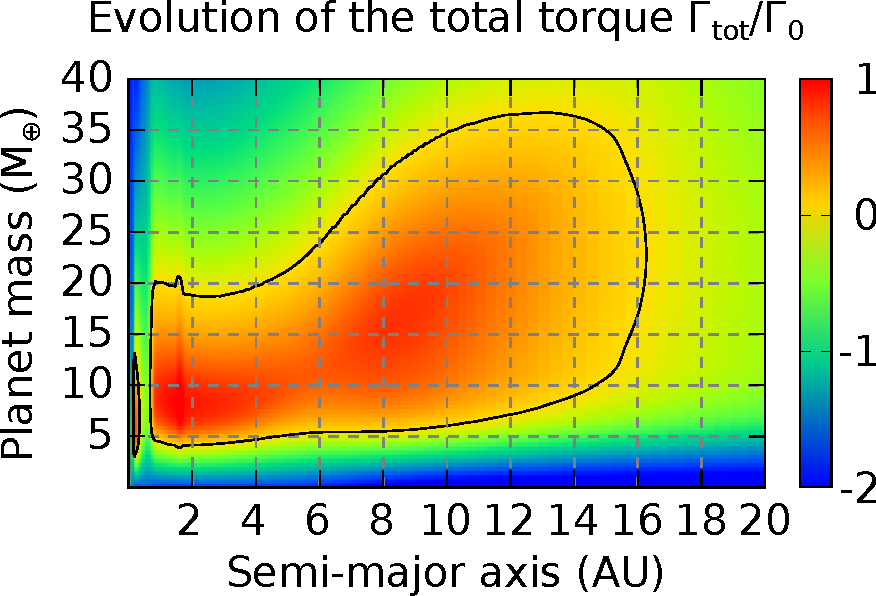
\includegraphics[width=0.65\linewidth]{figure/HSE/HSE_migration_map.pdf}
\caption{Cette carte représente l'effet du disque sur une planète en fonction de sa position en abscisse et de sa masse en ordonnée. La ligne noire représente la zone de couple nul, c'est à dire une zone où la migration de la planète s'arrête. Cette carte n'est valable que pour des planètes sur des orbites circulaires ($e\ll1$), c'est à dire quand l'amortissement du couple de corotation par l'excentricité est négligeable.}\label{fig:migration_map_HSE}
\end{figure}

Un zoom sur le bord interne du disque \reffig{fig:HSE_mig_zoom-in} montre la zone de couple positif juste avant le bord interne, dû à la décroissance rapide de la densité de surface et l'important couple de corotation qu'il engendre.

\begin{figure}[htb]
\centering
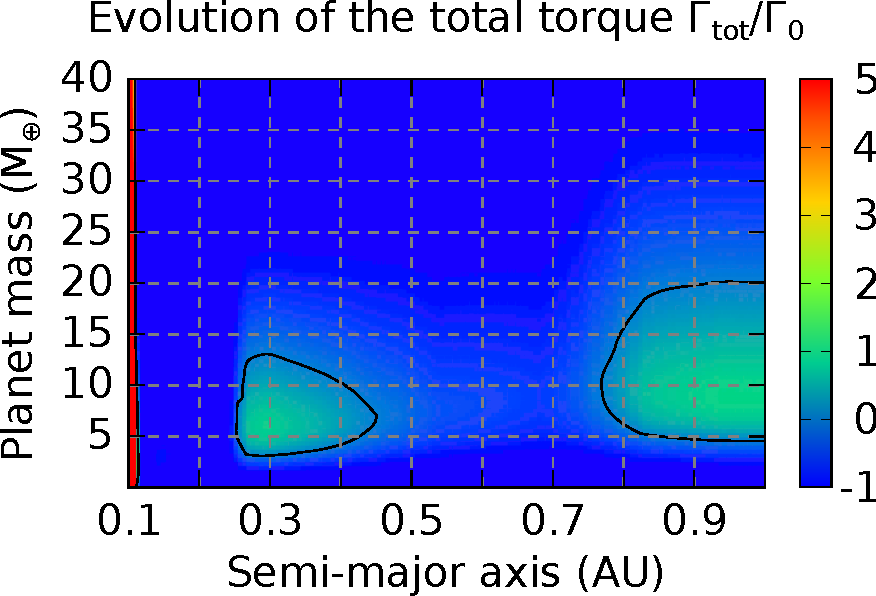
\includegraphics[width=0.65\linewidth]{figure/HSE/HSE_zoom-in.pdf}
\caption{Cette carte représente la migration d'une planète près du bord interne en fonction de sa position en abscisse et de sa masse en ordonnée. La ligne noire représente la zone de couple nul, c'est à dire une zone où la migration de la planète s'arrête. Cette carte n'est valable que pour des planètes sur des orbites circulaires ($e\ll1$), c'est à dire quand l'amortissement du couple de corotation par l'excentricité est négligeable.}\label{fig:HSE_mig_zoom-in}
\end{figure}

\subsection{Conditions initiales}
Initialement dans le système, on génère des embryons dont la masse varie de $0.1$ à $2\mearth$, pour une masse totale allant de $30$ à $100\mearth$. Des masses aléatoires différentes d'un embryon à l'autre permettent d'éviter les biais dûs aux masses égales. En effet, deux embryons de même masse migrent à la même vitesse, ce qui n'a aucune raison physique de se produire systématiquement dans un disque. Deux planètes migrant à la même vitesse ne peuvent pas entrer en collision, ou se placer en résonance, deux évènements cruciaux pour notre mécanisme de formation. 

De plus, quand deux corps sont en résonance, il y a un effet du rapport de masse sur les niveaux réciproques d'excentricité. Des masses égales maximisent les perturbations gravitationnelle de deux corps en résonance \refsec{sec:mass-ratio-effect}. Quand ce n'est pas le cas, le plus gros corps est celui qui a l'excentricité la plus faible, mais c'est aussi celui qui impose la stabilisation du système de deux corps là où lui ressent le couple du disque le plus faible.
%TODO parler du fait qu'il ne faut pas prendre des masses fixes, expliquer pourquoi. Montrer des statistiques de simulations. 

\subsection{Systèmes possibles}
En dessous d'une certaine masse limite qui dépend des paramètres du disque mais qui se situe généralement entre $2$ et $10\mearth$, les planètes migrent toutes vers l'intérieur, quelle que soit leur position initiale dans le disque. Pour le disque considéré ici \reffig{fig:migration_map_HSE}, cette limite se situe environ à $4\mearth$.

L'évolution peut suivre deux cas de figures différents, mais non exclusifs.

Dans un premier cas, les embryons migrent vers l'intérieur et il n'y a pas suffisamment de collisions durant leur migration pour qu'ils puissent migrer vers l'extérieur à un quelconque moment. On se trouve alors dans le cas d'une formation au bord interne décrite \refsec{sec:inner_edge_formation}. 

Dans un deuxième cas, une ou plusieurs planètes grossissent suffisamment par collision pour ressentir un couple positif vers l'extérieur. Plusieurs sous-cas de figures sont alors possibles, décrits \refsec{sec:outward-case}.

\subsubsection{Formation au bord interne : systèmes compacts}\label{sec:inner_edge_formation}
Des embryons migrent vers l'intérieur, de manière isolée ou par vague de sous-systèmes en résonance.

En raison de la diminution rapide de la densité de surface près du bord interne, la planète ressent un fort couple positif principalement dû au couple de corotation \reffig{fig:HSE_mig_zoom-in}. 

Un système de planètes en résonance se forme alors, les planètes internes migrant vers l'extérieur, les planètes externes migrant elles vers l'intérieur. Ce système en résonance va naturellement chercher à s'équilibrer. Cet équilibre est dicté par le fait que chaque planète ressent un couple non nul, elle possède aussi une excentricité à cause des autres corps en résonance, et ce système compact est continuellement soumis à des perturbations d'autant plus importantes que le nombre de corps en résonance est grand. 

Des collisions et réarrangements ont alors lieu, diminuant ainsi le nombre de corps et augmentant la stabilité du système global. 

\bigskip

Certaines planètes peuvent entrer dans la cavité interne du disque, poussées par le système non encore stabilisé. Elles ne perçoivent alors plus aucun effet du disque, que ce soit la migration ou l'amortissement de l'excentricité et de l'inclinaison. Dans ce cas de figure, elles peuvent ne plus être en résonance avec le reste du système. 

Même si durant l'évolution, il est possible que la planète la plus interne sorte du disque, entre en collision avec l'étoile centrale, ou soit ejectée, il est très facile de maintenir un système compact au bord interne en raison du fort couple positif qui va s'exercer sur le planète la plus interne du système alors que ce dernier cherche à migrer vers l'intérieur.

\subsubsection{Migration vers l'extérieur : candidats de planètes géantes}\label{sec:outward-case}
Lors de la migration vers l'intérieur de tous les embryons, il est possible pour une planète de grossir suffisamment vite pour ressentir un couple positif. Ce couple positif est censé entrainer une migration vers l'extérieur de la planète, ce serait systématiquement le cas si cette dernière était isolée. Mais dans son voisinage se trouvent d'autres planètes qui elles migrent vers l'intérieur. Très rapidement la planète va entrer en résonance avec un embryon planétaire qui migre vers l'intérieur.

L'effet décrit \refsec{sec:shifted_CZ} s'applique alors. La migration différentielle et le rapport de masse ont ici une importance capitale. Si la différence de vitesse est trop grande, alors les deux planètes ne peuvent pas former un système en résonance. La résonance est rapidement cassée et les deux corps continuent leur migration. Ceci est d'autant plus vrai si le rapport de masse est important, car la brève augmentation d'excentricité qui a lieu lors d'une capture en résonance n'aura que peu d'effet sur la plus grosse planète. Cette dernière sera très peu sensible aux perturbations gravitationnelle de son compagnon résonant et continuera sa migration vers l'extérieur sans quasiment ralentir. 

\begin{figure}[htb]
\centering
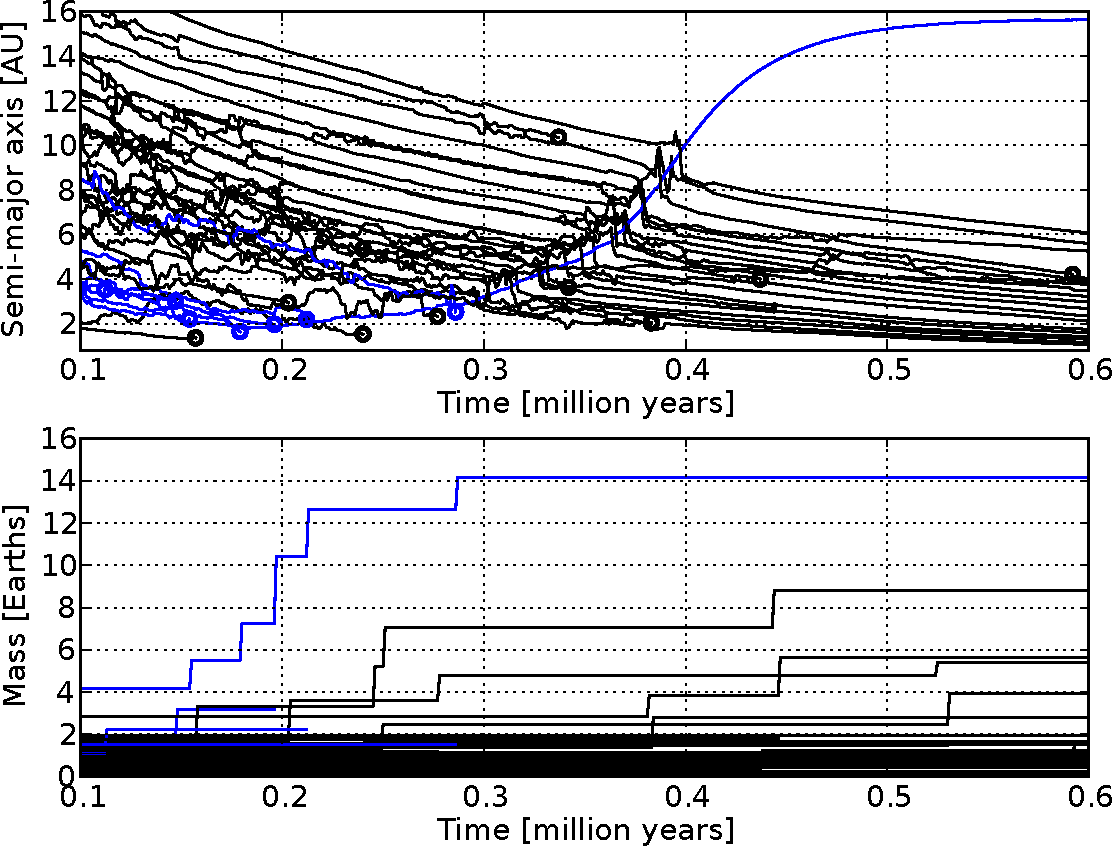
\includegraphics[width=0.65\linewidth]{figure/HSE/single_outward.pdf}
\caption{Formation d'un cœur de planète géante. La planète dont l'évolution est notée en bleu devient massive suffisamment vite pour pouvoir migrer vers l'extérieur. Les cercles représentent des collisions. Les autres courbes bleu qui disparaissent sont des embryons qui rentrent en collision avec la planète considérée et fusionnent avec elle. }\label{fig:single_outward}%/sse/cossou/HSE/disk_param/300_05/simu00010
\end{figure}

\reffig{fig:single_outward} illustre ce scénario. Cette dernière atteint par collisions la masse de $6\mearth$ au bout de $300 000\unit{ans}$ alors qu'elle se trouve à $1.2\unit{AU}$ ce qui est suffisant pour qu'elle puisse migrer vers l'extérieur. Cependant, les perturbations gravitationnelles des autres corps qui eux migrent vers l'intérieur l'empêchent de se comporter comme une planète isolée. Dans les quelques dizaines de milliers d'années suivants, 3 nouvelles collisions ont lieu. La planète fait maintenant $13\mearth$. La différence de masse avec ses voisins immédiats lui permet de migrer vers l'extérieur malgré les perturbations résonantes qui augmentent son excentricité. Comme détaillé \refsec{sec:mass-ratio-effect}, plus le rapport de masse est important, et plus la migration est dominée par la planète massive. Dans un système résonant avec rapport de masse élevé, la petite planète a une excentricité importante, son couple de corotation est fortement atténué, ce qui n'est pas le cas de la planète 
massive. Cette dernière migre comme si elle n'était pas en résonance, et à partir de là, soit elle emporte le système avec elle, soit, comme dans le cas présent, la résonance fini par se briser et les deux planètes continuent leur migration séparément.

Dans la suite de la simulation, la planète est trop massive pour être arrêtée. La planète massive migrant vers l'extérieur, elle capture en résonance un embryon de faible masse. Les deux planètes migrent alors vers l'extérieur, emportées par la migration de la planète la plus massive. Pourtant le système n'est pas stable. Les perturbations finissent par briser le système de deux planètes qui a alors deux possibilités. Soit une collision survient, augmentant sa masse, soit la brève rencontre se termine par un échange d'orbite. Dans cet exemple, les deux planètes continuent leur migration séparément.

À la fin de la simulation, la planète de $17.4\mearth$ est à sa zone de couple nul, à $15.7\unit{AU}$. 

\bigskip

Il est aussi possible pour la planète migrant vers l'extérieur de capturer en résonance une planète dans une configuration stable, comme le montre \reffig{fig:2-body_outward}.
\begin{figure}[htb]
\centering
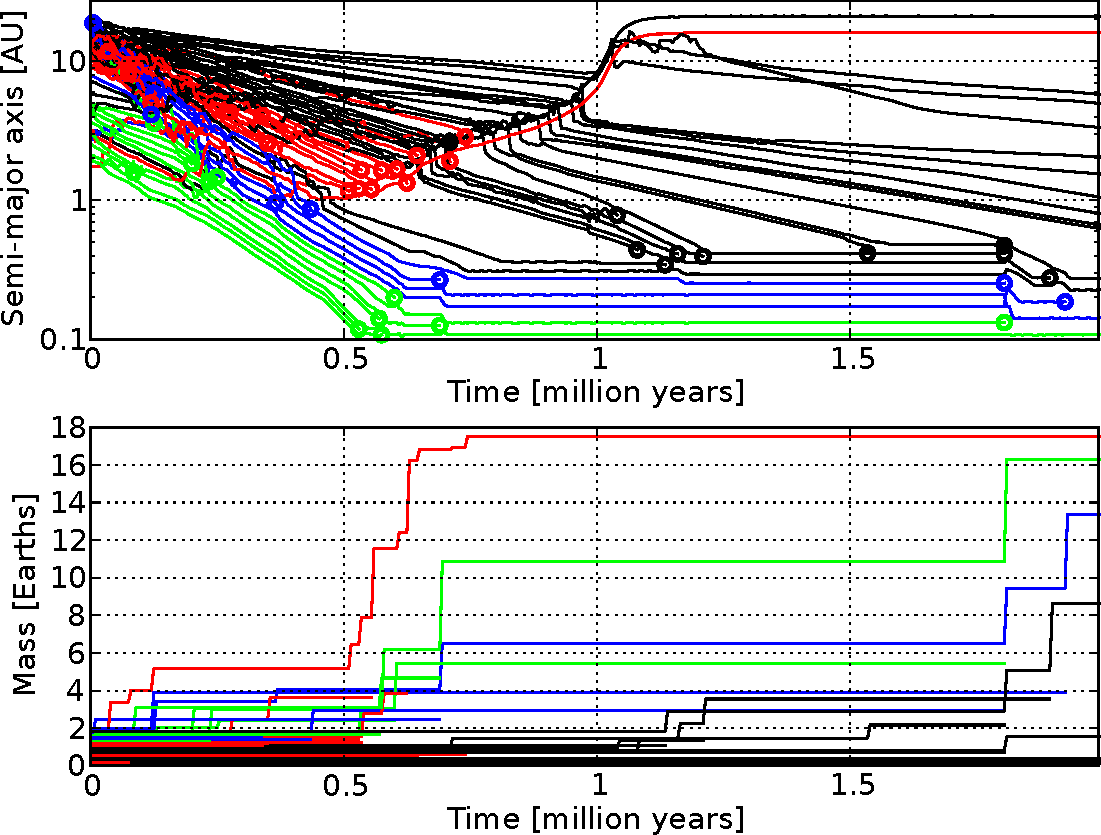
\includegraphics[width=0.65\linewidth]{figure/HSE/2-body_outward.pdf}
\caption{Formation d'un cœur de planète géante (en rouge) qui capture en résonance une planète de faible masse migrant très lentement vers l'intérieur.}\label{fig:2-body_outward}%/sse/cossou/HSE/disk_param/300_05/simu00038
\end{figure}

Dans cette même simulation, deux autres planètes massives sont formées (en vert et bleu) au bord interne, mais elles n'étaient pas massives suffisamment tôt pour migrer vers l'intérieur. Ainsi le même mécanisme, par un simple effet de timing, permet de créer soit des systèmes compacts de super terres chaudes, soit des embryons de planète géante qui pourront accréter du gaz dans les parties externes du disques, au delà de la ligne des glaces.

\bigskip

On a enfin un troisième et dernier cas où une planète grossit suffisamment rapidement pour migrer vers l'extérieur, mais est entrainée vers l'intérieur en étant capturée en résonance avec une planète de l'ordre de sa propre masse ce qui inverse son sens de migration. 

%TODO regarder la simulation %/sse/cossou/HSE/disk_param/300_05/simu00001/hires pour celà

%TODO chercher un cas où j'ai un système résonant à l'extérieur

%TODO chercher un cas où j'ai une planète qui grossi rapidement, qui veut migrer vers l'extérieur mais qui est emportéer à l'intérieur.

\subsection{Discussion}
Quand les embryons sont plus petits qu'une certaine masse critique dépendant des propriétés du disque, la migration est systématiquement vers l'intérieur. Un système compact de planètes qui grossissent par collisions se forme alors au bord interne qui retient ce système par le fort couple de corotation positif qui s'exerce juste avant le bord interne en raison de la forte décroissante de la densité de surface \citep{masset2006disk}.
%TODO le fait que le couple de lindblad est alors principalement égale au couple externe très fortement négatif ne suffit pas à contrebalancer le couple de corotation très positif. 

Pendant la migration vers l'intérieur, si un embryon grossit suffisamment vite, il peut commencer à migrer vers l'intérieur. Durant cette migration, des résonances vont se former avec les corps qui migrent pour la plupart vers l'intérieur. Par excitation résonante, la migration vers l'extérieur peut être ralentie voire stoppée, et les planètes peuvent de nouveau migrer vers l'intérieur. 

Pourtant, dans certains cas, une planète suffisamment massive peut migrer vers l'intérieur, emprisonnant des corps plus petits dans des résonances orbitales, avant de se placer à une zone de couple nul dans les parties externes du disque (dans celui présenté ici, vers $15\unit{UA}$.

\bigskip

Ce mécanisme peut alors former conjointement des systèmes compacts de super terres, proches du bord interne, ou des cœurs de planètes géantes dans les parties externes, avec possiblement des planètes beaucoup plus petites en résonance. 

La seule différence entre le cas système compact et le cas planète géante est le timing. 

En effet, il y a deux points importants. D'une part les embryons de faibles masses migrent vers l'intérieur quelle que soit leur position initiale. De plus, les embryons en dessous d'une certaine distance migrent tous vers l'intérieur quelle que soit leur masse. Les planètes qui ne répondent pas à ces critères migreront inexorablement vers le bord interne. 

Il faut donc dans le cas présent qu'un embryon atteigne la masse critique de $5\mearth$ au delà de $1\unit{UA}$ pour pouvoir migrer vers l'extérieur et devenir un cœur de planète géante.

\bigskip

Quand nous parlons ici de système compact, il faut garder à l'esprit que le disque est toujours présent. Nous ne faisons pas évoluer le disque au cours du temps, la dissipation aura donc certainement un effet. Les résonances, présentes systématiquement au bord interne à cause de la migration, auront des chances de disparaître si des déstabilisations surviennent pendant la dissipation. En effet, le système n'est stable qu'à cause de la dissipation induite par le disque de gaz. Pourtant, il est difficile de conclure car la manière dont le disque est dissipé aura une incidence sur la configuration finale du système. 

Ensuite, nous n'avons pas tenu compte de l'accrétion de gaz sur les super terres. D'un coté des planètes de plusieurs masses terrestres vont pouvoir accréter du gaz, mais la proximité de ces planètes à leur étoile centrale pourra avoir une effet dissipatif sur leur atmosphère. 

Ensuite, \cite{terquem2007migration} ont montré que la formation de systèmes compacts est possible. Ici, le modèle que nous avons repris est très similaire à leur modèle, à ceci près que nous avons modélisé la migration de manière consistante avec le disque (avec possibilité de couple positif et négatif en fonction de la masse et de la position de la planète). 

Ce que notre modèle montre en plus du modèle de \cite{terquem2007migration}, c'est que même avec migration vers l'extérieur, des systèmes compacts peuvent se former au bord interne, avec des propriétés très similaires aux propriétés des systèmes observés. Mais de plus, dans le même modèle, la formation de cœurs de planètes géantes dans les parties externes est possible. 

\section{Effets des paramètres du disque}
%TODO see kretke2012importance
%TODO regarder le papier de Bitsch 2013 et celui de 2012 où il regarde l'influence de l'indice adiabatique

Jusqu'à présent, je me suis concentré sur des cas particuliers. Dans le cas de la formation de super-Terres, je n'ai montré qu'un seul disque \refsec{sec:4.2}. Dans le cas du décalage de la zone de convergence, j'ai montré un disque artificiel modélisant une zone de convergence \refsec{sec:shifted_CZ}. 

Je vais montrer dans les paragraphes qui suivent que la migration est extrêmement sensible aux paramètres du disque.

\cite{kretke2012importance} ont déjà étudié l'influence des paramètres du disque sur la migration. Cependant, s'ils ont inclus des effets fins sur le bord interne et la migration, l'opacité est par exemple une simple loi de puissance. Nous montrerons que l'opacité est un paramètre sensible du modèle et qu'il est important de la modéliser le plus finement possible. 

\cite{bitsch2013influence} ont étudié en particulier l'effet de la viscosité $\nu$ et l'indice adiabatique $\gamma$ sur la migration dans le disque, au travers de simulations 3D. 


%TODO continuer

%TODO 
\subsection{Viscosité du disque}

%TODO 

Le couple de migration est sensible à la valeur de la viscosité $\nu$. En particulier, c'est le temps de diffusion visqueux qui modifie le niveau de saturation de la zone de corotation, et donc la valeur du couple de corotation. 

Pourtant, la carte de migration possède une deuxième sensibilité au modèle de viscosité. Selon que l'on choisi une viscosité constante ou une prescription alpha dans laquelle la viscosité $\nu$ croit avec la distance, cela a une influence sur l'évolution du couple en fonction de la position dans le disque. 

\subsection{Profil de densité de surface}
%TODO 
\subsection{Profil de température}
%TODO 
\subsection{Masse du disque}
%TODO 
\subsection{Table d'opacité}\label{sec:influence_opacity_table}
Le modèle utilisé pour déterminer les opacités dans un disque est bien souvent à peine nommé, et très peu discuté. Pourtant,
l'opacité est une grandeur physique qui a une influence très importante sur la physique du disque et la migration des planètes. 

Dans toute la suite, quand je parlerai de table d'opacité, je désigne le fait d'utiliser un tableau à deux dimensions,
proposant des valeurs de l'opacité pour différentes températures et densité. La table d'opacité est donc définie ici par
opposition à ce que j'appelle des lois d'opacité, modèles dans lesquels l'opacité est définie par des lois de puissance,
fonction de la température et de la densité, dans différents régimes de température et densité.

Ainsi une table d'opacité est simplement une tabulation de l'opacité, alors qu'une loi d'opacité correspond à un ajustement par
une loi de puissance. 

\bigskip

Généralement, c'est la loi d'opacité \cite{bell1994FU} qui est utilisée, aussi bien dans les simulations hydrodynamiques 2D et
3D que dans les simulations N-corps. 

Une autre loi d'opacité existante est \cite{zhu2009nonsteady}, loi quelque peu améliorée par rapport à \cite{bell1994FU},
l'augmentation des capacités des ordinateurs ayant permis de faire des calculs plus précis. 

De plus, nous utilisons aussi le modèle d'opacité très simple décrit par \cite{chambers2009analytic} dans lequel l'opacité est
constante et égale à $\kappa=3$ jusqu'à $1380\unit{K}$ où une transition s'opère vers une loi de puissance. Ce modèle nous
permet de voir l'effet d'un modèle par rapport à un cas où l'opacité est constante. En effet, dans le cas d'un disque
protoplanétaire, seules les régions les plus internes sont susceptibles d'atteindre des températures supérieures à
$1000\unit{K}$. 

Enfin, j'ai souhaité comparer ces deux lois d'opacité avec une table d'opacité, \cite{hure2000transition}. Cette table
d'opacité de Rosseland correspond à la composition suivante $X=0.70$, $Y=0.28$ et $Z=0.02$ et est basée sur
\cite{seaton1994opacities, alexander1994low, henning1996dust}.

\begin{figure}[htb]
\centering
\subfloat[\citep{bell1994FU}]{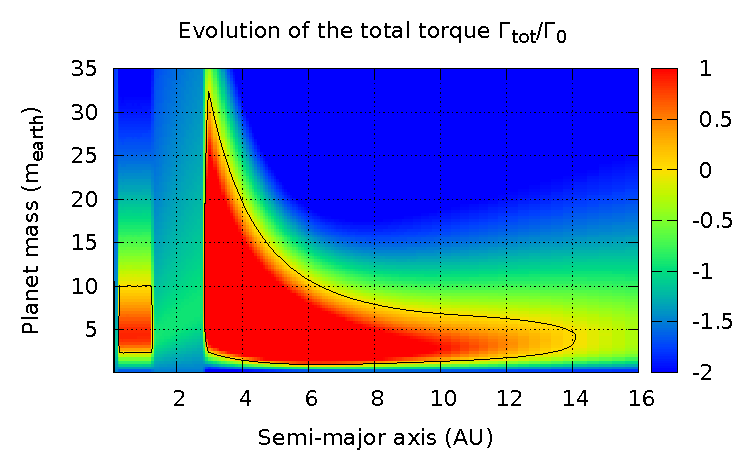
\includegraphics[width=0.49\textwidth]{figure/migration_map/opacity/opacity_bell.pdf}}\hfill
\subfloat[\citep{chambers2009analytic}]{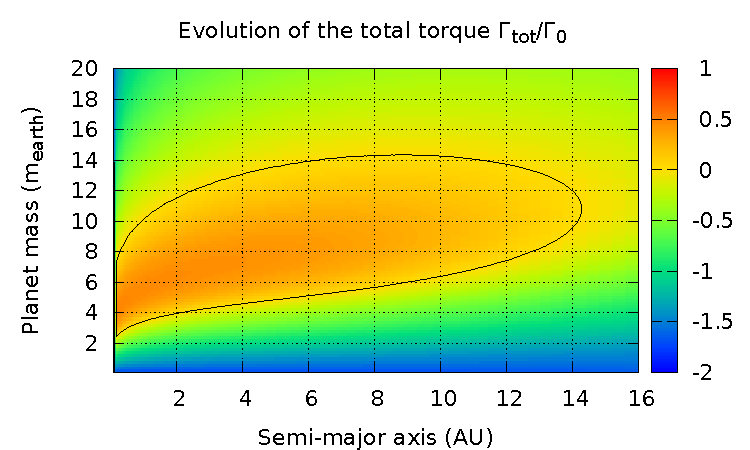
\includegraphics[width=0.49\textwidth]{%
figure/migration_map/opacity/opacity_chambers.pdf}}

\subfloat[\citep{zhu2009nonsteady}]{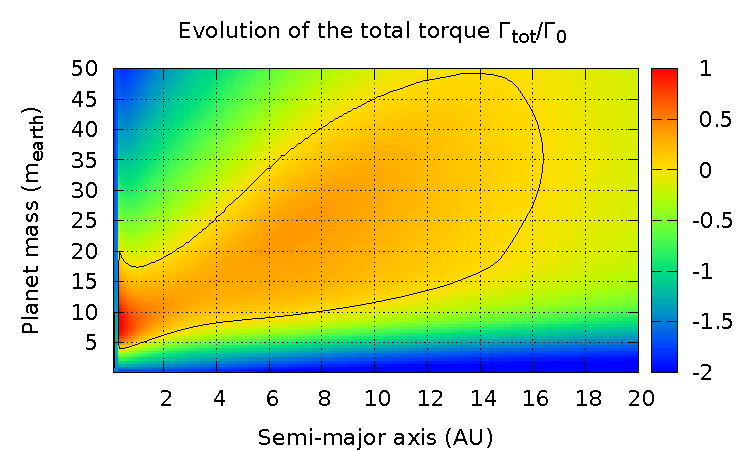
\includegraphics[width=0.49\textwidth]{figure/migration_map/opacity/opacity_zhu.pdf}}\hfill
\subfloat[\citep{hure2000transition}]{\label{fig:opacity_hure}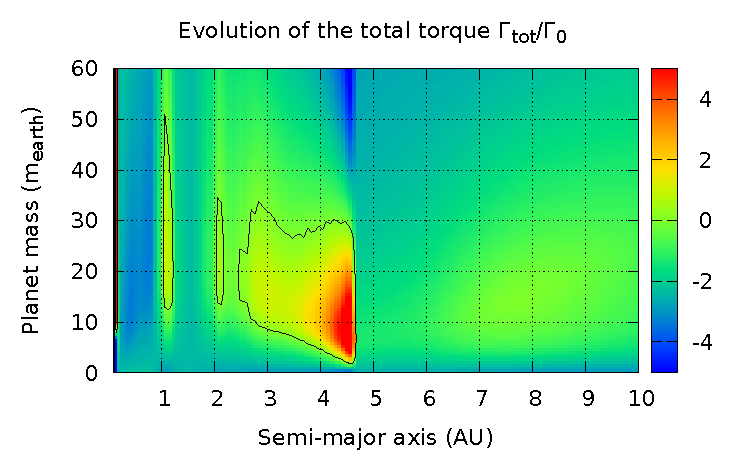
\includegraphics[width=0.49\textwidth]{%
figure/migration_map/opacity/opacity_hure.pdf}}
\caption{Cartes de migration obtenues pour le même disque, mais avec un modèle d'opacité différent. L'irradiation ayant un
effet important sur la carte de migration, elle a été désactivée ici afin de mieux mettre en valeur les différences entre
les modèles d'opacités. Notez que les échelles ne sont pas identiques.}
\end{figure}\label{fig:opacity_tables}

\reffig{fig:opacity_tables} montre les différentes cartes de migration que l'on obtient avec le même disque de référence mais
pour les 4 modèles d'opacité considérés. 

On considère la carte avec la table d'opacité \reffig{fig:opacity_hure} comme référence. En effet, les lois d'opacités utilisent
une table d'opacité en amont à partir de laquelle elles déduisent des lois de puissances par morceau afin de reproduire au mieux
la table d'opacité. La table d'opacité se traduit par une carte de migration complexe où chaque aspect de la table se traduit
sur la carte par une variation brutale de la migration. L'opacité a une grande influence sur la migration, que ce soit au
niveau du temps de diffusion qui régi la saturation que vis à vis du profil de température.

L'importance de l'opacité se manifeste au travers du temps de diffusion radiatif. Une opacité plus grande induit un temps de
diffusion radiatif plus important. 

On constate par ailleurs que les lois d'opacité lissent fortement la carte de migration (comparer la carte pour la table
d'opacité d'\cite{hure2000transition} avec les 3 autres). Notons en particulier une transition d'opacité dans \cite{bell1994FU}
qui n'existe pas dans les autres modèles et qui entraine une zone de convergence indépendante de la masse (dans le cas présent
à $1.3\unit{UA}$). Cette transition d'opacité, liée à l'évaporation des grains de glace d'eau, n'est en effet introduite que
dans ce modèle, les autres modèles considérant qu'elle n'illustre aucune réalité physique 
%TODO Ref sur la transition d'opacité fantome

Le modèle d'opacité choisi a donc une grande influence sur la carte de migration et donc le comportement des planètes dans un
disque. À l'heure actuelle, compte tenu de la puissance des ordinateurs, le choix d'une loi d'opacité par rapport à une table
d'opacité ne se justifie absolument plus. En effet, les approximations supplémentaires qu'engendrent une loi d'opacité comparé
à une table brute ne sont absolument pas compensées par le gain de temps de calcul que cela engendre. Dans mon cas, la routine
implémentant la table d'opacité est même plus rapide que la routine pour les lois d'opacités. La seule différence est qu'il
faut stocker un tableau contenant la table d'opacité, ce qui n'est absolument pas limitatif avec les ordinateurs actuels.

Les modèles d'opacités étant une source d'incertitude pour toutes les simulations numériques, que ce soit des simulations
N-corps ou des simulations hydrodynamiques 2D ou 3D, je pense qu'il est important d'apporter une attention particulière au
choix du modèle. 

À l'heure actuelle, dans le cas particulier de la migration planétaire, la valeur de l'opacité ainsi que la pente qu'elle
engendre sur le profil de température sont des sources importantes d'incertitudes. Il pourrait être intéressant de réaliser une
étude d'envergure afin de réaliser une table d'opacité tenant compte des nouvelles capacités des ordinateurs, afin de coller au
mieux à ce que l'on sait des disques. 

Il restera pourtant toujours des incertitudes quant aux propriétés des poussières, taille et quantité, ainsi que son évolution
au cours du temps. La poussière étant une source majeure d'opacité dans le disque, son évolution au cours du temps doit avoir
une influence toute aussi majeure que nous ne pouvons que négliger à l'heure actuelle malgré les implications que cela peut
avoir sur la formation des planètes.

%TODO

\subsection{Effet de l'irradiation}
En choisissant ou non d'inclure l'irradiation dans l'équation de l'énergie permettant de calculer le profil de température, on
change de manière importante la carte de migration. 

\begin{figure}[htb]
\centering
\subfloat[Avec irradiation]{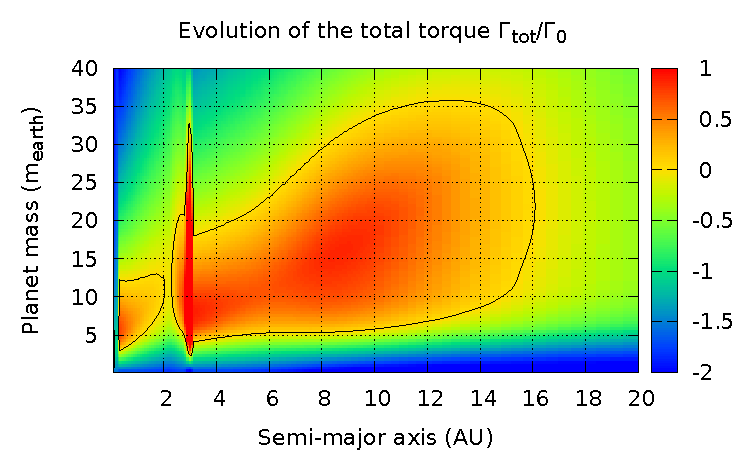
\includegraphics[width=0.49\textwidth]{figure/migration_map/bell_irr.pdf}}\hfill
\subfloat[Sans irradiation]{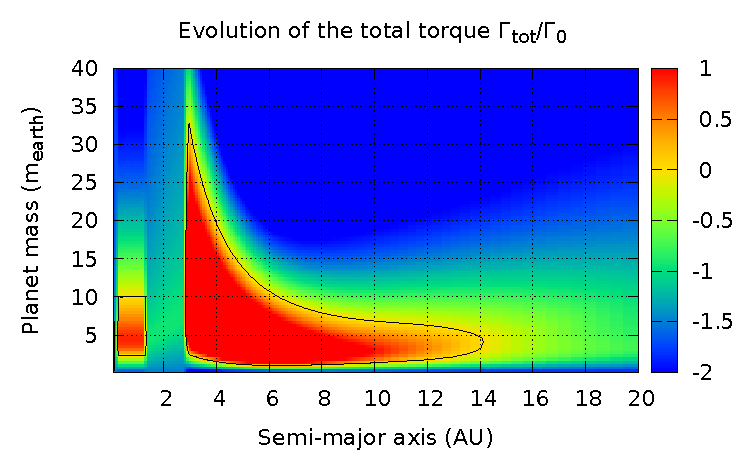
\includegraphics[width=0.49\textwidth]{%
figure/migration_map/bell_noirr.pdf}}

\caption{Influence de l'irradiation sur la carte de migration à travers le profil de température. Afin de visualiser plus
facilement les effets, \cite{bell1994FU} a été utilisé pour l'opacité.}\label{fig:irradiation}
\end{figure}

Afin de visualiser l'effet de l'irradiation, nous avons utilisé les lois d'opacités de \cite{bell1994FU}. En effet,
le principal effet de l'irradiation est de lisser le profil de température. Sans irradiation, une transition d'opacité marquée
comme celles de \cite{bell1994FU} se répercute directement sur le profil de température \reffig{fig:temp_profile_irradiation}.
On voit donc apparaître des zone de convergences dues à des transitions d'opacités qui sont totalement déformées par
l'irradiation comme on peut le constater sur \reffig{fig:irradiation}.

\begin{figure}[htb]
\centering
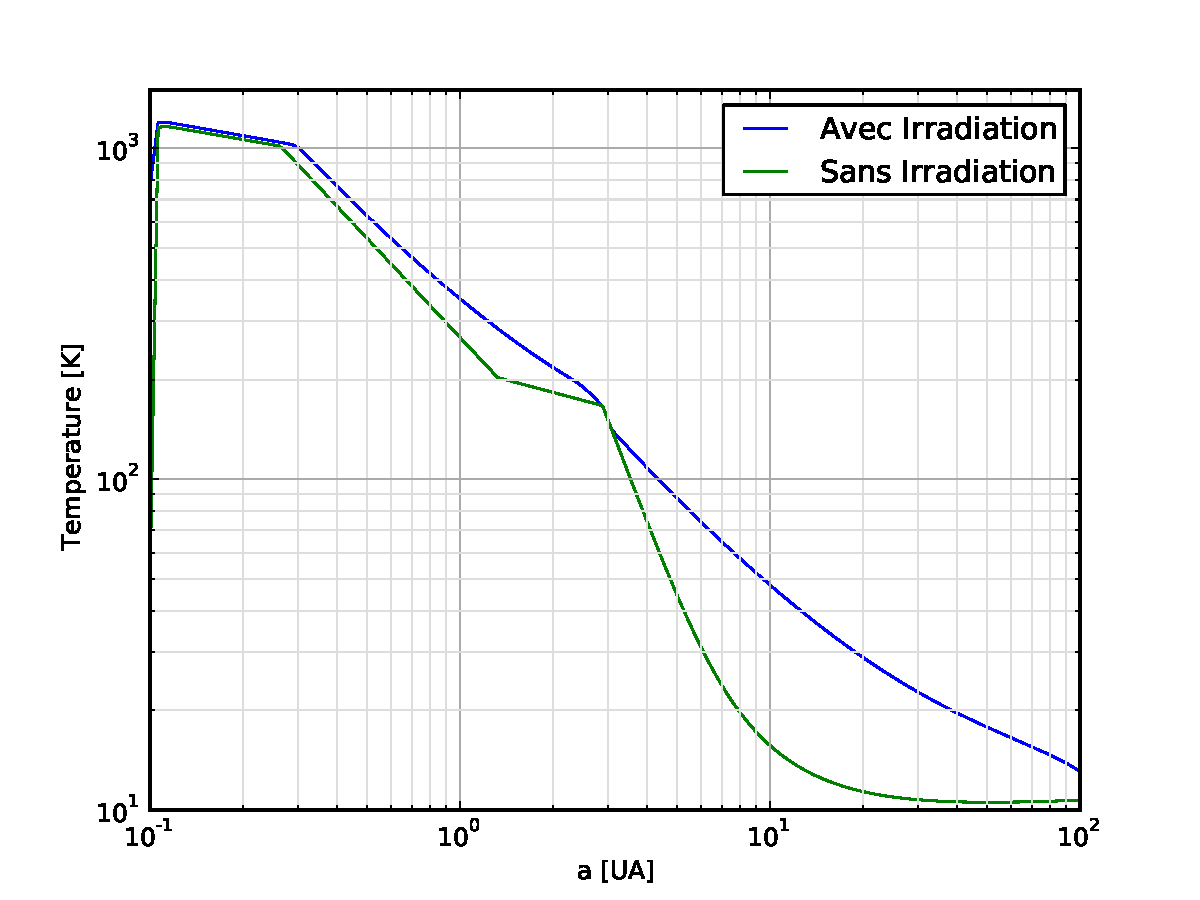
\includegraphics[width=0.6\linewidth]{figure/migration_map/temperature_with_irradiation.pdf}
\caption{Profil de température avec ou sans irradiation. L'irradiation est calculée avec les paramètres $T_\star =
5700\unit{K}$, $R_\star = 4.65\cdot 10^-3\unit{AU}$, disk albedo $\varepsilon =
0.5$.}\label{fig:temp_profile_irradiation}
\end{figure}

Ainsi, sans irradiation, les deux transitions d'opacités à $1.3$ et $2.9\unit{UA}$ induisent un changement brutal de la pente
du profil de température, ce qui a pour effet de changer le sens de migration (de positif à négatif, puis l'inverse).

Dans les parties externes, l'irradiation a pour effet de diminuer la pente du profil de température qui tend vers un profil en
$R^{-0.5}$ quand le disque est purement passif.

%TODO expliquer pourquoi les parties externes ``montent'' en masse. En clair, au lieu d'avoir une décroissance de la zone de
% couple nul avec la masse, c'est l'inverse qui se produit quand on active l'irradiation.

\subsection{Longueur de lissage}
Dans les modèles numériques des disques protoplanétaires, le potentiel gravitationnel doit être modifié afin ne pas diverger aux très faibles distances mutuelles. En particulier, des problèmes peuvent survenir quand on modélise des objets, tels des planètes, par des masses ponctuelles. 

De même, dans le cas de simulations hydrodynamiques 2D, le modèle se base sur des moyennes azimutales des différentes quantités physiques. Le lissage du potentiel gravitationnel est ici nécessaire afin de diluer la densité de surface et reproduire au mieux l'aspect 3D du disque. On comprend alors aisément que la longueur de lissage va être reliée à l'échelle de hauteur du disque qui est elle aussi une mesure de l'extension azimutale du disque. 

Plusieurs groupes ont cherché à étudier la longueur de lissage en détail, en particulier pour trouver la valeur optimale à utiliser \citep{hure2009local, muller2012treating}. Ces études cherchent à trouver la longueur de lissage qui permet de reproduire les simulations 3D à l'aide des simulations 2D. 

Une longueur de lissage relativement importante $b/h = 0.75$ est nécessaire pour reproduire correctement le couple de Lindblad \citep{masset2002coorbital}. Pour le couple de corotation, la zone fer-à-cheval étant très proche de la planète, ce dernier est extrêmement sensible à la longueur de lissage. En effet, \cite{masset2002coorbital} a montré que dans certains cas le couple de corotation pouvait être plus d'un ordre de grandeur plus important en fonction de la valeur du lissage que l'on applique. La valeur préconisée est alors autour de $b/h\sim 0.5-0.6$. Ainsi, \cite{masset2002coorbital} conclue qu'il est peu probable de trouver une valeur optimale pour la longueur de lissage, les valeurs optimales pour les couples de Lindblad et de corotation étant incompatible. 

\cite{muller2012treating} suggère d'utiliser une longueur de lissage $b/h = 0.7$ tout en notant que des différences notables subsistent avec les simulations 3D. 

\cite{hure2009local}, en étudiant des disques sans planètes conseillent la plage de valeur suivante $0.13 \lesssim b/h \lesssim 0.29$.

\bigskip

\cite{paardekooper2010torque, paardekooper2011torque} et les formules analytiques ou semi-analytiques qu'ils fournissent pour
décrire la migration de type I (\refeq{eq:lindblad-torque}, \refeq{eq:saturated-corotation-torque},
\refeq{eq:linear-corotation-torque}) introduisent une telle dépendance. 

\begin{figure}[htb]
\centering
\subfloat[$b/h = 0.2$]{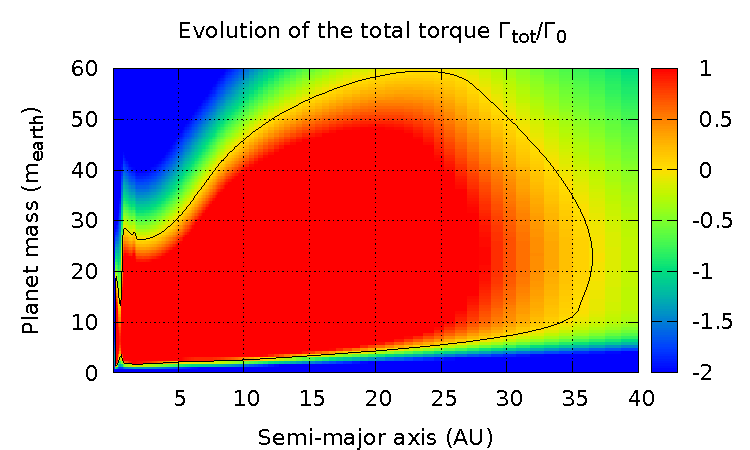
\includegraphics[width=0.49\textwidth]{figure/migration_map/smoothing/smoothing_0_2.pdf}}\hfill
\subfloat[$b/h = 0.4$]{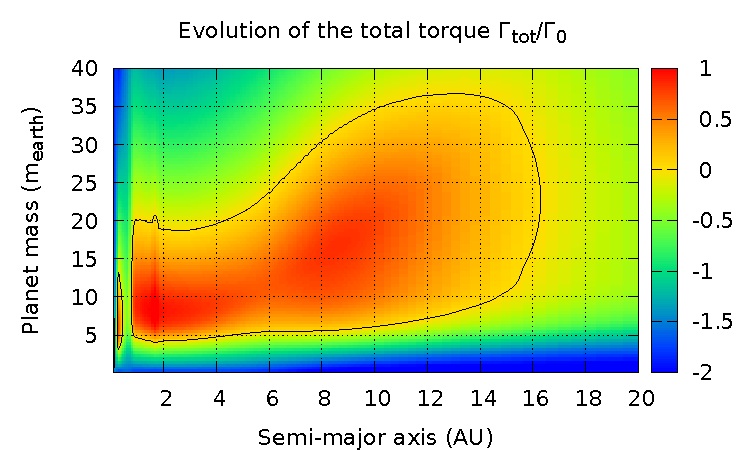
\includegraphics[width=0.49\textwidth]{figure/migration_map/smoothing/smoothing_0_4.pdf}}\\
\subfloat[$b/h = 0.6$]{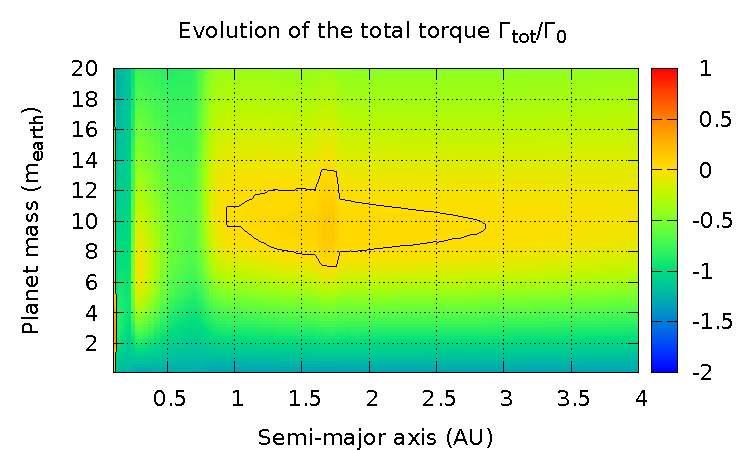
\includegraphics[width=0.49\textwidth]{figure/migration_map/smoothing/smoothing_0_6.pdf}}\hfill
\subfloat[$b/h = 0.7$]{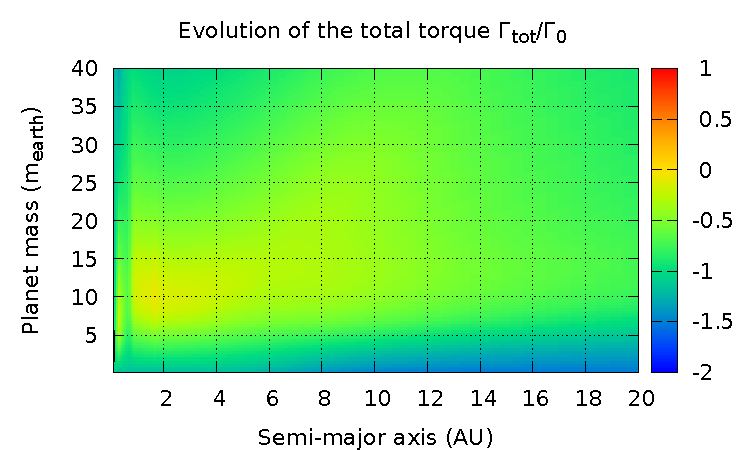
\includegraphics[width=0.49\textwidth]{figure/migration_map/smoothing/smoothing_0_7.pdf}}\\
\caption{Effet de la longueur de lissage $b/h$ du potentiel gravitationnel sur la carte de migration du disque de référence. Ici seule la longueur de lissage change.  Pour plus de détails sur les cartes de migration \refsec{sec:migrations-maps}.}\label{fig:migration_map_smoothing}
\end{figure}

\reffig{fig:migration_map_smoothing} montre qu'en fonction de la longueur de lissage, on peut se trouver dans un cas où il y a migration systématique vers l'intérieur ($b/h=0.7$) ou migration quasi systématique vers l'extérieur ($b/h=0.2$). Si une valeur de $0.2$ semble peu réaliste au regard de la migration planétaire \citep{muller2012treating}, il est courant de voir des simulations effectuées avec $b/h=0.3-0.6$ \citep{masset2002coorbital, devalborro2006comparative, paardekooper2009corotation}. 

Une longueur de lissage $0.6 \leqslant b/h \leqslant 0.76$ sous estime le couple de corotation et sur-estime le couple de Lindblad \citep{masset2002coorbital}. Même si les valeurs préconisées par les études de sensibilités se situent autour de $0.6-0.7$, les études faisant des simulations hydrodynamiques utilisent plus couramment une valeur de $b/h=0.4$ \citep{paardekooper2011torque}. Il n'existe donc pas de valeur optimale pour la longueur de lissage quand le disque que l'on modélise est utilisé pour étudier la migration planétaire. Si cette section ne conclue pas quant à une valeur à utiliser pour $b/h$ c'est avant tout pour insister sur le fait que la seule conclusion à tirer, c'est que la longueur de lissage est une source importance d'incertitude dans nos modèles. Une longueur de lissage importante (resp. faible) a tendance à favoriser la migration vers l'intérieur (resp. l'extérieur). 

\begin{figure}[htb]
\centering
\subfloat[$b/h = 0.5$]{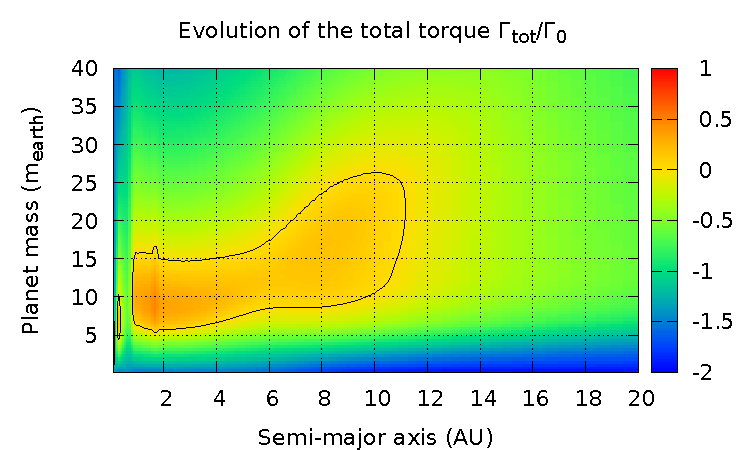
\includegraphics[width=0.49\textwidth]{figure/migration_map/smoothing/smoothing_0_5.pdf}}\hfill
\subfloat[$b/h = 0.76$ pour $\Gamma_L$ et $0.5$ pour $\Gamma_C$]{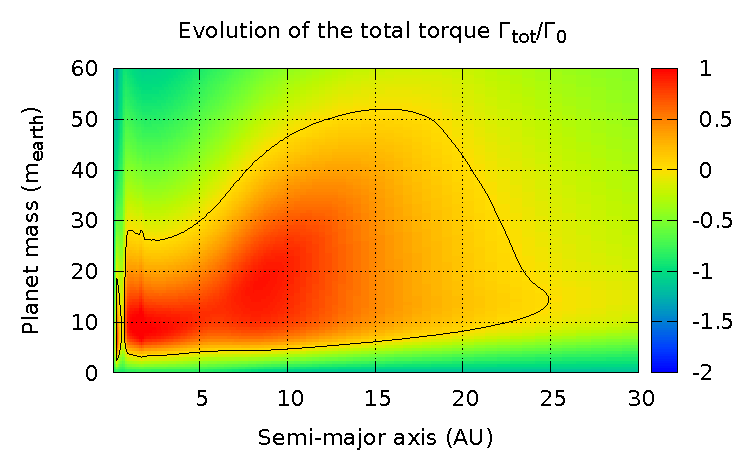
\includegraphics[width=0.49\textwidth]{figure/migration_map/smoothing/smoothing_0_5_modified.pdf}}
\caption{Comparaison d'un cas où la longueur de lissage est fixée à $b/h=0.5$, et d'un autre cas où la longueur de lissage a été fixée à $0.76$ pour le couple de Lindblad et à $0.5$ pour le couple de Corotation, correspondant aux valeurs conseillées pour les deux couples séparés \citep{masset2002coorbital}. Pour plus de détails sur les cartes de migration \refsec{sec:migrations-maps}.}\label{fig:modified_smoothing}
\end{figure}

Inclure des formules pour la migration de type I nous offre une liberté supplémentaire par rapport aux simulations hydrodynamique, celle de fixer une longueur de lissage $b/h$ différente pour le couple de Lindblad et pour le couple de Corotation. Suivant les prescriptions données par \cite{masset2002coorbital} j'ai donc calculé la carte de migration d'une simulation où je fixe une longueur de lissage $b/h=0.76$ pour le couple de Lindblad, et une longueur de lissage $b/h=0.5$ pour le couple de Corotation. J'obtiens alors les cartes représentées \reffig{fig:modified_smoothing}, toujours dans le cas du disque de référence. %TODO décrire le disque de référence en section 3, et en particulier penser à emttre une référence ici vers la bonne section.

%TODO proposer cette idée d'utiliser une longueur de lissage différente pour lindblad et corotation? En discuter avec Sean et Arnaud.


%TODO parler du travail d'audrey? Je voudrais en parler avec elle, lui montrer cette section et savoir ce qu'elle en pense. 
% En particulier, j'aimerais discuter avec elle du fait que la longueur de lissage qu'elle calcule ne peut pas s'appliquer dans
mon cas à moi. J'aimerais voir si elle saurait m'expliquer pourquoi (dans mon cas j'ai une planète, et pas elle)

\subsection{Masse moléculaire moyenne}
La masse moléculaire moyenne $\mu$ va varier dans le disque, principalement à cause de l'évaporation de certaines
espèces chimiques à différentes températures. La plupart sont totalement négligeable vu leur abondance limitée. Le problème
aurait pu se poser au bord interne du disque, où la température est très importante. Dans cette région là, la masse moléculaire
moyenne peut varier à cause de la photodissociation de la molécule $\mathrm{H_2}$. En supposant que le rapport d'abondance
$\mathrm{He/H}=0.1$, la masse moléculaire, initialement de $\mu=2.35$ passe alors à environ $\mu\sim 1.3$

\begin{figure}[htb]
\centering
\subfloat[$\mu=2.35$]{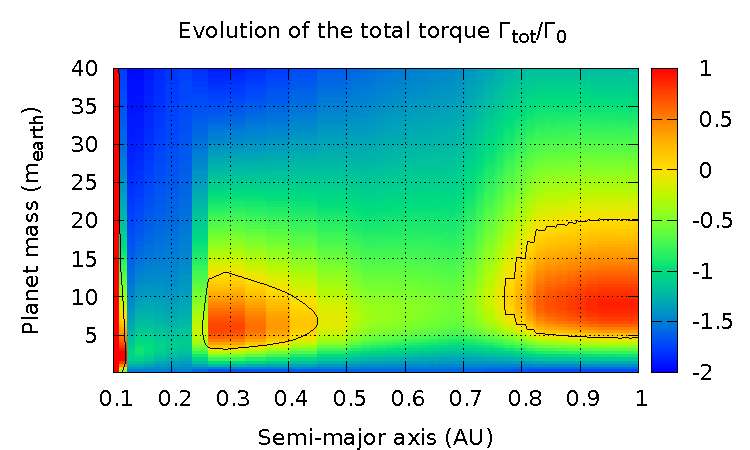
\includegraphics[width=0.49\textwidth]{figure/migration_map/mmw_fully_molecular.pdf}}\hfill
\subfloat[$\mu=1.3$]{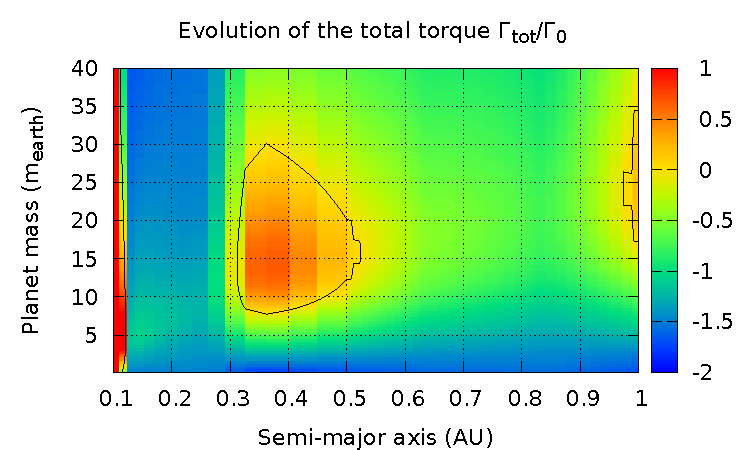
\includegraphics[width=0.49\textwidth]{figure/migration_map/mmw_HI.pdf}}
\caption{Influence de la masse moléculaire moyenne $\mu$ sur la carte de migration. Seules les
parties très internes du disque sont ici représentées. Le même disque est utilisé, seule la masse
moléculaire change afin de refléter l'influence de la photodissociation de $\mathrm{H_2}$ en
$\mathrm{HI}$ quand la température devient importante. }\label{fig:migration_map_mmw}
\end{figure}

\reffig{fig:migration_map_mmw} montre l'influence de la masse moléculaire moyenne sur la carte de migration pour un disque
donné. On s'attend à ce que la photodissociation de $\mathrm{H_2}$ ne devienne importante que dans les parties très internes,
bien en dessous de $1\unit{UA}$. Dans ces régions là, on constate que la variation de la masse moléculaire moyenne n'a que peu
d'effet. Il ne nous est donc pas apparu important de prendre cette variation en compte, les changements induits sur la carte de
migration étant bien inférieur à l'influence du modèle d'opacité par exemple. Cette effet nous parait donc totalement
négligeable au regard des incertitudes de notre modèle.
